\batchmode
\documentclass[a4paper]{book}
\usepackage{a4wide}
\usepackage{makeidx}
\usepackage{graphicx}
\usepackage{multicol}
\usepackage{float}
\usepackage{listings}
\usepackage{color}
\usepackage{textcomp}
\usepackage{alltt}
\usepackage{times}
\usepackage{ifpdf}
\ifpdf
\usepackage[pdftex,
            pagebackref=true,
            colorlinks=true,
            linkcolor=blue,
            unicode
           ]{hyperref}
\else
\usepackage[ps2pdf,
            pagebackref=true,
            colorlinks=true,
            linkcolor=blue,
            unicode
           ]{hyperref}
\usepackage{pspicture}
\fi
\usepackage[utf8]{inputenc}
\usepackage{doxygen}
\lstset{language=C++,inputencoding=utf8,basicstyle=\footnotesize,breaklines=true,breakatwhitespace=true,tabsize=4,numbers=left }
\makeindex
\setcounter{tocdepth}{3}
\renewcommand{\footrulewidth}{0.4pt}
\begin{document}
\hypersetup{pageanchor=false}
\begin{titlepage}
\vspace*{7cm}
\begin{center}
{\Large haigo \\[1ex]\large 0.1 }\\
\vspace*{1cm}
{\large Generated by Doxygen 1.7.1}\\
\vspace*{0.5cm}
{\small Tue Jan 24 2012 09:35:23}\\
\end{center}
\end{titlepage}
\clearemptydoublepage
\pagenumbering{roman}
\tableofcontents
\clearemptydoublepage
\pagenumbering{arabic}
\hypersetup{pageanchor=true}
\chapter{HaiGo v.0.1}
\label{index}\hypertarget{index}{}This is just a placeholder text.

\begin{DoxyAuthor}{Author}
Clemens Dorner 
\end{DoxyAuthor}
\begin{DoxyVersion}{Version}
0.1 
\end{DoxyVersion}
\begin{DoxyDate}{Date}
2012-\/01-\/22 
\end{DoxyDate}

\chapter{Todo List}
\label{todo}
\hypertarget{todo}{}
\label{todo__todo000002}
\hypertarget{todo__todo000002}{}
 
\begin{DoxyDescription}
\item[Class \hyperlink{structcommand__func}{command\_\-func} ]Check if function declaration needs parameters! 
\end{DoxyDescription}

\label{todo__todo000004}
\hypertarget{todo__todo000004}{}
 
\begin{DoxyDescription}
\item[Global \hyperlink{group___g_t_p___core___play___commands_ga16a060c01868977200be0b381b03c6f9}{gtp\_\-play}(int gtp\_\-argc, char gtp\_\-argv\mbox{[}\mbox{]}\mbox{[}MAX\_\-TOKEN\_\-LENGTH\mbox{]}) ]Description is missing!

Remove captured stones here ... 

Update move history ... 
\end{DoxyDescription}

\label{todo__todo000003}
\hypertarget{todo__todo000003}{}
 
\begin{DoxyDescription}
\item[Global \hyperlink{group___g_t_p___debug___commands_ga7c297f28150386dc85b1de08e6f8d456}{gtp\_\-showboard}(int gtp\_\-argc, char gtp\_\-argv\mbox{[}\mbox{]}\mbox{[}MAX\_\-TOKEN\_\-LENGTH\mbox{]}) ]These functions have to be implemmted: gtp\_\-genmove, gtp\_\-undo.
\begin{DoxyItemize}
\item void gtp\_\-genmove( int argc, char argv\mbox{[}\mbox{]}\mbox{[}MAX\_\-TOKEN\_\-LENGTH\mbox{]} );
\item void gtp\_\-undo( int argc, char argv\mbox{[}\mbox{]}\mbox{[}MAX\_\-TOKEN\_\-LENGTH\mbox{]} ); 
\end{DoxyItemize}
\end{DoxyDescription}

\label{todo__todo000001}
\hypertarget{todo__todo000001}{}
 
\begin{DoxyDescription}
\item[Global \hyperlink{board_8h_ac70f31e9f413033ba999d4eccb459cb5}{init\_\-board}(int wanted\_\-board\_\-size) ]A size check has to be implemented probably. 
\end{DoxyDescription}
\chapter{Module Index}
\section{Modules}
Here is a list of all modules:\begin{DoxyCompactList}
\item \contentsline{section}{Go Text Protocol Commands}{\pageref{group___g_t_p___commands}}{}
\begin{DoxyCompactList}
\item \contentsline{section}{Go Text Protocol Administrative Commands}{\pageref{group___g_t_p___administrative___commands}}{}
\item \contentsline{section}{Go Text Protocol Setup Commands}{\pageref{group___g_t_p___setup___commands}}{}
\item \contentsline{section}{Go Text Protocol Core Play Commands}{\pageref{group___g_t_p___core___play___commands}}{}
\item \contentsline{section}{Go Text Protocol Debug Commands}{\pageref{group___g_t_p___debug___commands}}{}
\end{DoxyCompactList}
\end{DoxyCompactList}

\chapter{Data Structure Index}
\section{Data Structures}
Here are the data structures with brief descriptions:\begin{DoxyCompactList}
\item\contentsline{section}{\hyperlink{structcommand}{command} }{\pageref{structcommand}}{}
\item\contentsline{section}{\hyperlink{structcommand__func}{command\_\-func} (Connects one given command name with proper function pointer )}{\pageref{structcommand__func}}{}
\end{DoxyCompactList}

\chapter{File Index}
\section{File List}
Here is a list of all files with brief descriptions:\begin{DoxyCompactList}
\item\contentsline{section}{src/\hyperlink{board_8c}{board.c} }{\pageref{board_8c}}{}
\item\contentsline{section}{src/\hyperlink{board_8h}{board.h} }{\pageref{board_8h}}{}
\item\contentsline{section}{src/\hyperlink{global__const_8h}{global\_\-const.h} }{\pageref{global__const_8h}}{}
\item\contentsline{section}{src/\hyperlink{global__tools_8c}{global\_\-tools.c} }{\pageref{global__tools_8c}}{}
\item\contentsline{section}{src/\hyperlink{global__tools_8h}{global\_\-tools.h} }{\pageref{global__tools_8h}}{}
\item\contentsline{section}{src/\hyperlink{io_8c}{io.c} }{\pageref{io_8c}}{}
\item\contentsline{section}{src/\hyperlink{io_8h}{io.h} }{\pageref{io_8h}}{}
\item\contentsline{section}{src/\hyperlink{main_8c}{main.c} }{\pageref{main_8c}}{}
\item\contentsline{section}{src/\hyperlink{run__program_8c}{run\_\-program.c} }{\pageref{run__program_8c}}{}
\item\contentsline{section}{src/\hyperlink{run__program_8h}{run\_\-program.h} }{\pageref{run__program_8h}}{}
\end{DoxyCompactList}

\chapter{Module Documentation}
\hypertarget{group___g_t_p___commands}{
\section{Go Text Protocol Commands}
\label{group___g_t_p___commands}\index{Go Text Protocol Commands@{Go Text Protocol Commands}}
}


Collaboration diagram for Go Text Protocol Commands:\nopagebreak
\begin{figure}[H]
\begin{center}
\leavevmode
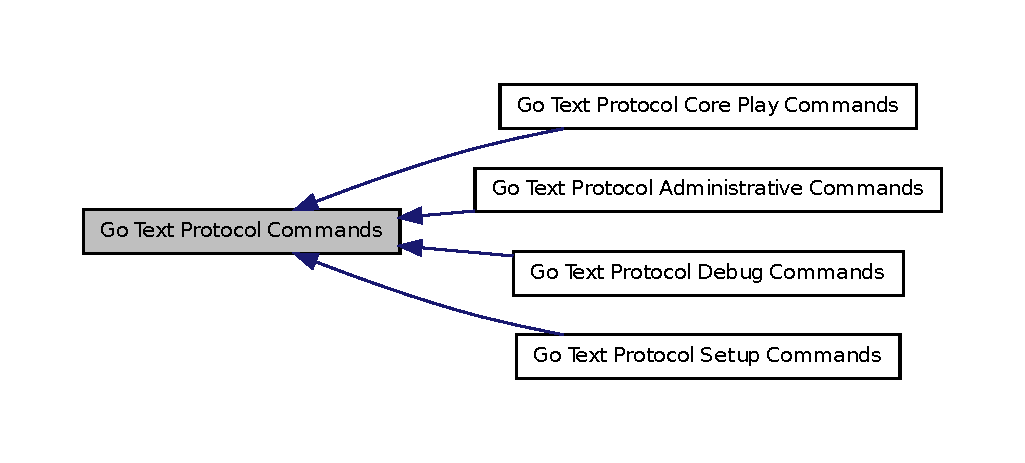
\includegraphics[width=400pt]{group___g_t_p___commands}
\end{center}
\end{figure}


\subsection*{Modules}
\begin{DoxyCompactItemize}
\item 
\hyperlink{group___g_t_p___administrative___commands}{Go Text Protocol Administrative Commands}
\item 
\hyperlink{group___g_t_p___setup___commands}{Go Text Protocol Setup Commands}
\item 
\hyperlink{group___g_t_p___core___play___commands}{Go Text Protocol Core Play Commands}
\item 
\hyperlink{group___g_t_p___debug___commands}{Go Text Protocol Debug Commands}
\end{DoxyCompactItemize}


\subsection{Detailed Description}
The following functions are implemented as defined in the Go Text Protocol version 2 
\hypertarget{group___g_t_p___administrative___commands}{
\section{Go Text Protocol Administrative Commands}
\label{group___g_t_p___administrative___commands}\index{Go Text Protocol Administrative Commands@{Go Text Protocol Administrative Commands}}
}


Collaboration diagram for Go Text Protocol Administrative Commands:\nopagebreak
\begin{figure}[H]
\begin{center}
\leavevmode
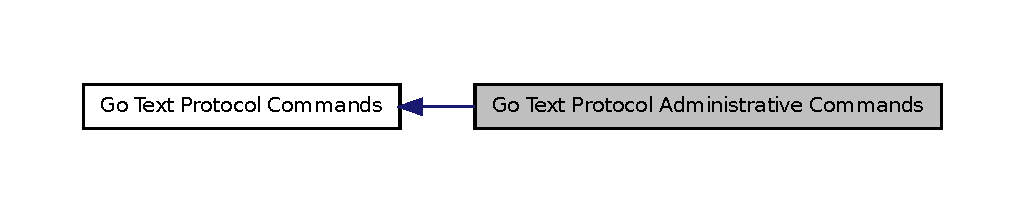
\includegraphics[width=400pt]{group___g_t_p___administrative___commands}
\end{center}
\end{figure}


\subsection*{Functions}
\begin{DoxyCompactItemize}
\item 
void \hyperlink{group___g_t_p___administrative___commands_ga625849e565ca8f4e13fc521165d73910}{gtp\_\-quit} (int gtp\_\-argc, char gtp\_\-argv\mbox{[}$\,$\mbox{]}\mbox{[}MAX\_\-TOKEN\_\-LENGTH\mbox{]})
\begin{DoxyCompactList}\small\item\em Quits the program. \item\end{DoxyCompactList}\item 
void \hyperlink{group___g_t_p___administrative___commands_ga264cb45ac6de56306d1006a4ee8a1f4d}{gtp\_\-version} (int gtp\_\-argc, char gtp\_\-argv\mbox{[}$\,$\mbox{]}\mbox{[}MAX\_\-TOKEN\_\-LENGTH\mbox{]})
\begin{DoxyCompactList}\small\item\em Shows the program's version number. \item\end{DoxyCompactList}\item 
void \hyperlink{group___g_t_p___administrative___commands_ga57d397237b5bc6129ada6cdcfeaa9aad}{gtp\_\-protocol\_\-version} (int gtp\_\-argc, char gtp\_\-argv\mbox{[}$\,$\mbox{]}\mbox{[}MAX\_\-TOKEN\_\-LENGTH\mbox{]})
\begin{DoxyCompactList}\small\item\em Shows the used GTP version number. \item\end{DoxyCompactList}\item 
void \hyperlink{group___g_t_p___administrative___commands_ga493e544f8b83dd08fb5ebf25c127fb60}{gtp\_\-name} (int gtp\_\-argc, char gtp\_\-argv\mbox{[}$\,$\mbox{]}\mbox{[}MAX\_\-TOKEN\_\-LENGTH\mbox{]})
\begin{DoxyCompactList}\small\item\em Shows the program's name. \item\end{DoxyCompactList}\item 
void \hyperlink{group___g_t_p___administrative___commands_gac1f9e22691e53c8b8aa46d473008c262}{gtp\_\-known\_\-command} (int gtp\_\-argc, char gtp\_\-argv\mbox{[}$\,$\mbox{]}\mbox{[}MAX\_\-TOKEN\_\-LENGTH\mbox{]})
\begin{DoxyCompactList}\small\item\em Shows whether a given GTP command is implemented or not. \item\end{DoxyCompactList}\item 
void \hyperlink{group___g_t_p___administrative___commands_gabe46d9c2f68c87415a2550ec8358c664}{gtp\_\-list\_\-commands} (int gtp\_\-argc, char gtp\_\-argv\mbox{[}$\,$\mbox{]}\mbox{[}MAX\_\-TOKEN\_\-LENGTH\mbox{]})
\begin{DoxyCompactList}\small\item\em Shows a list of all know GTP commands. \item\end{DoxyCompactList}\end{DoxyCompactItemize}


\subsection{Function Documentation}
\hypertarget{group___g_t_p___administrative___commands_gac1f9e22691e53c8b8aa46d473008c262}{
\index{GTP\_\-Administrative\_\-Commands@{GTP\_\-Administrative\_\-Commands}!gtp\_\-known\_\-command@{gtp\_\-known\_\-command}}
\index{gtp\_\-known\_\-command@{gtp\_\-known\_\-command}!GTP_Administrative_Commands@{GTP\_\-Administrative\_\-Commands}}
\subsubsection[{gtp\_\-known\_\-command}]{\setlength{\rightskip}{0pt plus 5cm}void gtp\_\-known\_\-command (
\begin{DoxyParamCaption}
\item[{int}]{ gtp\_\-argc, }
\item[{char}]{ gtp\_\-argv\mbox{[}$\,$\mbox{]}\mbox{[}MAX\_\-TOKEN\_\-LENGTH\mbox{]}}
\end{DoxyParamCaption}
)}}
\label{group___g_t_p___administrative___commands_gac1f9e22691e53c8b8aa46d473008c262}


Shows whether a given GTP command is implemented or not. 

\hyperlink{group___g_t_p___administrative___commands_gac1f9e22691e53c8b8aa46d473008c262}{gtp\_\-known\_\-command()} $<$command\_\-name$>$ returns either the string \char`\"{}true\char`\"{} or \char`\"{}false\char`\"{} therefore showing whether a given GTP command is known or not.


\begin{DoxyParams}{Parameters}
\item[\mbox{\tt[in]} {\em gtp\_\-argc}]Number of arguments of GTP command \item[\mbox{\tt[in]} {\em gtp\_\-argv}]Array of all arguments for GTP command \end{DoxyParams}
\begin{DoxyReturn}{Returns}
\char`\"{}true\char`\"{} $|$ \char`\"{}false\char`\"{} 
\end{DoxyReturn}
\begin{DoxySeeAlso}{See also}
Go Text Protokol version 2, 6.3.1 Administrative Commands 
\end{DoxySeeAlso}


Definition at line 390 of file run\_\-program.c.




\begin{DoxyCode}
{
    int  i;
    bool is_command_known = false;

    if ( gtp_argc < 1 ) {
        set_output_error();
        add_output( "missing argument: command_name" );
        return;
    }
    if ( gtp_argc > 1 ) {
        set_output_error();
        add_output( "only one argument required: command_name" );
        return;
    }

    for ( i = 0; i < COUNT_KNOWN_COMMANDS; i++ ) {
        if ( strcmp( known_commands[i].command, gtp_argv[0] ) == 0 ) {
            is_command_known = true;
            break;
        }
    }

    if ( is_command_known == true ) {
        add_output("true");
    }
    else {
        add_output("false");
    }

    return;
}
\end{DoxyCode}


\hypertarget{group___g_t_p___administrative___commands_gabe46d9c2f68c87415a2550ec8358c664}{
\index{GTP\_\-Administrative\_\-Commands@{GTP\_\-Administrative\_\-Commands}!gtp\_\-list\_\-commands@{gtp\_\-list\_\-commands}}
\index{gtp\_\-list\_\-commands@{gtp\_\-list\_\-commands}!GTP_Administrative_Commands@{GTP\_\-Administrative\_\-Commands}}
\subsubsection[{gtp\_\-list\_\-commands}]{\setlength{\rightskip}{0pt plus 5cm}void gtp\_\-list\_\-commands (
\begin{DoxyParamCaption}
\item[{int}]{ gtp\_\-argc, }
\item[{char}]{ gtp\_\-argv\mbox{[}$\,$\mbox{]}\mbox{[}MAX\_\-TOKEN\_\-LENGTH\mbox{]}}
\end{DoxyParamCaption}
)}}
\label{group___g_t_p___administrative___commands_gabe46d9c2f68c87415a2550ec8358c664}


Shows a list of all know GTP commands. 

\hyperlink{group___g_t_p___administrative___commands_gabe46d9c2f68c87415a2550ec8358c664}{gtp\_\-list\_\-commands()} shows the name of the program as defined by PROGRAM\_\-NAME.


\begin{DoxyParams}{Parameters}
\item[\mbox{\tt[in]} {\em gtp\_\-argc}]Number of arguments of GTP command \item[\mbox{\tt[in]} {\em gtp\_\-argv}]Array of all arguments for GTP command \end{DoxyParams}
\begin{DoxyReturn}{Returns}
nothing 
\end{DoxyReturn}
\begin{DoxySeeAlso}{See also}
Go Text Protokol version 2, 6.3.1 Administrative Commands 
\end{DoxySeeAlso}


Definition at line 436 of file run\_\-program.c.




\begin{DoxyCode}
{
    int i;

    for ( i = 0; i < COUNT_KNOWN_COMMANDS; i++ ) {
        add_output( known_commands[i].command );
    }

    return;
}
\end{DoxyCode}


\hypertarget{group___g_t_p___administrative___commands_ga493e544f8b83dd08fb5ebf25c127fb60}{
\index{GTP\_\-Administrative\_\-Commands@{GTP\_\-Administrative\_\-Commands}!gtp\_\-name@{gtp\_\-name}}
\index{gtp\_\-name@{gtp\_\-name}!GTP_Administrative_Commands@{GTP\_\-Administrative\_\-Commands}}
\subsubsection[{gtp\_\-name}]{\setlength{\rightskip}{0pt plus 5cm}void gtp\_\-name (
\begin{DoxyParamCaption}
\item[{int}]{ gtp\_\-argc, }
\item[{char}]{ gtp\_\-argv\mbox{[}$\,$\mbox{]}\mbox{[}MAX\_\-TOKEN\_\-LENGTH\mbox{]}}
\end{DoxyParamCaption}
)}}
\label{group___g_t_p___administrative___commands_ga493e544f8b83dd08fb5ebf25c127fb60}


Shows the program's name. 

\hyperlink{group___g_t_p___administrative___commands_ga493e544f8b83dd08fb5ebf25c127fb60}{gtp\_\-name()} shows the name of the program as defined by PROGRAM\_\-NAME.


\begin{DoxyParams}{Parameters}
\item[\mbox{\tt[in]} {\em gtp\_\-argc}]Number of arguments of GTP command \item[\mbox{\tt[in]} {\em gtp\_\-argv}]Array of all arguments for GTP command \end{DoxyParams}
\begin{DoxyReturn}{Returns}
nothing 
\end{DoxyReturn}
\begin{DoxySeeAlso}{See also}
Go Text Protokol version 2, 6.3.1 Administrative Commands 
\end{DoxySeeAlso}


Definition at line 368 of file run\_\-program.c.




\begin{DoxyCode}
{

    add_output(PROGRAM_NAME);

    return;
}
\end{DoxyCode}


\hypertarget{group___g_t_p___administrative___commands_ga57d397237b5bc6129ada6cdcfeaa9aad}{
\index{GTP\_\-Administrative\_\-Commands@{GTP\_\-Administrative\_\-Commands}!gtp\_\-protocol\_\-version@{gtp\_\-protocol\_\-version}}
\index{gtp\_\-protocol\_\-version@{gtp\_\-protocol\_\-version}!GTP_Administrative_Commands@{GTP\_\-Administrative\_\-Commands}}
\subsubsection[{gtp\_\-protocol\_\-version}]{\setlength{\rightskip}{0pt plus 5cm}void gtp\_\-protocol\_\-version (
\begin{DoxyParamCaption}
\item[{int}]{ gtp\_\-argc, }
\item[{char}]{ gtp\_\-argv\mbox{[}$\,$\mbox{]}\mbox{[}MAX\_\-TOKEN\_\-LENGTH\mbox{]}}
\end{DoxyParamCaption}
)}}
\label{group___g_t_p___administrative___commands_ga57d397237b5bc6129ada6cdcfeaa9aad}


Shows the used GTP version number. 

\hyperlink{group___g_t_p___administrative___commands_ga57d397237b5bc6129ada6cdcfeaa9aad}{gtp\_\-protocol\_\-version()} shows the currently used Go Text Protocol version number. Currently this is version number 2 as defined in GTP\_\-VERSION.


\begin{DoxyParams}{Parameters}
\item[\mbox{\tt[in]} {\em gtp\_\-argc}]Number of arguments of GTP command \item[\mbox{\tt[in]} {\em gtp\_\-argv}]Array of all arguments for GTP command \end{DoxyParams}
\begin{DoxyReturn}{Returns}
nothing 
\end{DoxyReturn}
\begin{DoxySeeAlso}{See also}
Go Text Protokol version 2, 6.3.1 Administrative Commands 
\end{DoxySeeAlso}


Definition at line 348 of file run\_\-program.c.




\begin{DoxyCode}
{

    add_output(GTP_VERSION);

    return;
}
\end{DoxyCode}


\hypertarget{group___g_t_p___administrative___commands_ga625849e565ca8f4e13fc521165d73910}{
\index{GTP\_\-Administrative\_\-Commands@{GTP\_\-Administrative\_\-Commands}!gtp\_\-quit@{gtp\_\-quit}}
\index{gtp\_\-quit@{gtp\_\-quit}!GTP_Administrative_Commands@{GTP\_\-Administrative\_\-Commands}}
\subsubsection[{gtp\_\-quit}]{\setlength{\rightskip}{0pt plus 5cm}void gtp\_\-quit (
\begin{DoxyParamCaption}
\item[{int}]{ gtp\_\-argc, }
\item[{char}]{ gtp\_\-argv\mbox{[}$\,$\mbox{]}\mbox{[}MAX\_\-TOKEN\_\-LENGTH\mbox{]}}
\end{DoxyParamCaption}
)}}
\label{group___g_t_p___administrative___commands_ga625849e565ca8f4e13fc521165d73910}


Quits the program. 

\hyperlink{group___g_t_p___administrative___commands_ga625849e565ca8f4e13fc521165d73910}{gtp\_\-quit()} quits the whole program by calling \hyperlink{run__program_8c_a1e1c6b03caa51f0c2aa5879f82be64c9}{set\_\-quit\_\-program()}.


\begin{DoxyParams}{Parameters}
\item[\mbox{\tt[in]} {\em gtp\_\-argc}]Number of arguments of GTP command \item[\mbox{\tt[in]} {\em gtp\_\-argv}]Array of all arguments for GTP command \end{DoxyParams}
\begin{DoxyReturn}{Returns}
nothing 
\end{DoxyReturn}
\begin{DoxySeeAlso}{See also}
Go Text Protokol version 2, 6.3.1 Administrative Commands 
\end{DoxySeeAlso}


Definition at line 306 of file run\_\-program.c.




\begin{DoxyCode}
{

    set_quit_program();

    return;
}
\end{DoxyCode}


\hypertarget{group___g_t_p___administrative___commands_ga264cb45ac6de56306d1006a4ee8a1f4d}{
\index{GTP\_\-Administrative\_\-Commands@{GTP\_\-Administrative\_\-Commands}!gtp\_\-version@{gtp\_\-version}}
\index{gtp\_\-version@{gtp\_\-version}!GTP_Administrative_Commands@{GTP\_\-Administrative\_\-Commands}}
\subsubsection[{gtp\_\-version}]{\setlength{\rightskip}{0pt plus 5cm}void gtp\_\-version (
\begin{DoxyParamCaption}
\item[{int}]{ gtp\_\-argc, }
\item[{char}]{ gtp\_\-argv\mbox{[}$\,$\mbox{]}\mbox{[}MAX\_\-TOKEN\_\-LENGTH\mbox{]}}
\end{DoxyParamCaption}
)}}
\label{group___g_t_p___administrative___commands_ga264cb45ac6de56306d1006a4ee8a1f4d}


Shows the program's version number. 

\hyperlink{group___g_t_p___administrative___commands_ga264cb45ac6de56306d1006a4ee8a1f4d}{gtp\_\-version()} shows the version number as defined by PROGRAM\_\-VERSION.


\begin{DoxyParams}{Parameters}
\item[\mbox{\tt[in]} {\em gtp\_\-argc}]Number of arguments of GTP command \item[\mbox{\tt[in]} {\em gtp\_\-argv}]Array of all arguments for GTP command \end{DoxyParams}
\begin{DoxyReturn}{Returns}
nothing 
\end{DoxyReturn}
\begin{DoxySeeAlso}{See also}
Go Text Protokol version 2, 6.3.1 Administrative Commands 
\end{DoxySeeAlso}


Definition at line 326 of file run\_\-program.c.




\begin{DoxyCode}
{

    add_output(PROGRAM_VERSION);

    return;
}
\end{DoxyCode}



\hypertarget{group___g_t_p___setup___commands}{
\section{Go Text Protocol Setup Commands}
\label{group___g_t_p___setup___commands}\index{Go Text Protocol Setup Commands@{Go Text Protocol Setup Commands}}
}


Collaboration diagram for Go Text Protocol Setup Commands:\nopagebreak
\begin{figure}[H]
\begin{center}
\leavevmode
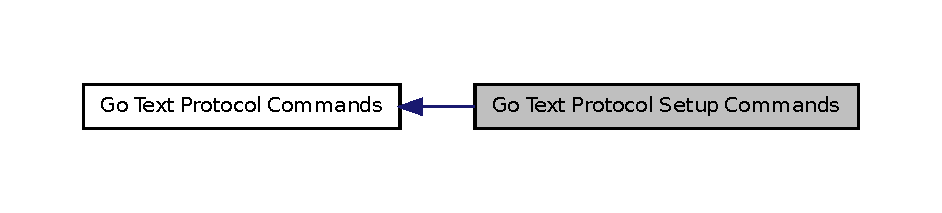
\includegraphics[width=400pt]{group___g_t_p___setup___commands}
\end{center}
\end{figure}


\subsection*{Functions}
\begin{DoxyCompactItemize}
\item 
void \hyperlink{group___g_t_p___setup___commands_ga79e2fa5bdce2dd440754746a2e35dd24}{gtp\_\-boardsize} (int gtp\_\-argc, char gtp\_\-argv\mbox{[}$\,$\mbox{]}\mbox{[}MAX\_\-TOKEN\_\-LENGTH\mbox{]})
\begin{DoxyCompactList}\small\item\em Changes the current board size. \item\end{DoxyCompactList}\item 
void \hyperlink{group___g_t_p___setup___commands_ga2a539d6423ba407b126487e12a6a222b}{gtp\_\-clear\_\-board} (int gtp\_\-argc, char gtp\_\-argv\mbox{[}$\,$\mbox{]}\mbox{[}MAX\_\-TOKEN\_\-LENGTH\mbox{]})
\begin{DoxyCompactList}\small\item\em Clears the board. \item\end{DoxyCompactList}\item 
void \hyperlink{group___g_t_p___setup___commands_ga9f823dc0dc9c21fabf4ba223fc515682}{gtp\_\-komi} (int gtp\_\-argc, char gtp\_\-argv\mbox{[}$\,$\mbox{]}\mbox{[}MAX\_\-TOKEN\_\-LENGTH\mbox{]})
\begin{DoxyCompactList}\small\item\em Sets komi. \item\end{DoxyCompactList}\end{DoxyCompactItemize}


\subsection{Function Documentation}
\hypertarget{group___g_t_p___setup___commands_ga79e2fa5bdce2dd440754746a2e35dd24}{
\index{GTP\_\-Setup\_\-Commands@{GTP\_\-Setup\_\-Commands}!gtp\_\-boardsize@{gtp\_\-boardsize}}
\index{gtp\_\-boardsize@{gtp\_\-boardsize}!GTP_Setup_Commands@{GTP\_\-Setup\_\-Commands}}
\subsubsection[{gtp\_\-boardsize}]{\setlength{\rightskip}{0pt plus 5cm}void gtp\_\-boardsize (
\begin{DoxyParamCaption}
\item[{int}]{ gtp\_\-argc, }
\item[{char}]{ gtp\_\-argv\mbox{[}$\,$\mbox{]}\mbox{[}MAX\_\-TOKEN\_\-LENGTH\mbox{]}}
\end{DoxyParamCaption}
)}}
\label{group___g_t_p___setup___commands_ga79e2fa5bdce2dd440754746a2e35dd24}


Changes the current board size. 

\hyperlink{group___g_t_p___setup___commands_ga79e2fa5bdce2dd440754746a2e35dd24}{gtp\_\-boardsize()} changes the current size of the board. by PROGRAM\_\-NAME.


\begin{DoxyParams}{Parameters}
\item[\mbox{\tt[in]} {\em gtp\_\-argc}]Number of arguments of GTP command \item[\mbox{\tt[in]} {\em gtp\_\-argv}]Array of all arguments for GTP command \end{DoxyParams}
\begin{DoxyReturn}{Returns}
nothing 
\end{DoxyReturn}
\begin{DoxySeeAlso}{See also}
Go Text Protokol version 2, 6.3.2 Setup Commands 
\end{DoxySeeAlso}


Definition at line 463 of file run\_\-program.c.




\begin{DoxyCode}
{
    int board_size = (int) atoi( gtp_argv[0] );

    if ( board_size < BOARD_SIZE_MIN || board_size > BOARD_SIZE_MAX ) {
        set_output_error();
        add_output("unacceptable size");
        return;
    }

    free_board();
    init_board(board_size);

    return;
}
\end{DoxyCode}


\hypertarget{group___g_t_p___setup___commands_ga2a539d6423ba407b126487e12a6a222b}{
\index{GTP\_\-Setup\_\-Commands@{GTP\_\-Setup\_\-Commands}!gtp\_\-clear\_\-board@{gtp\_\-clear\_\-board}}
\index{gtp\_\-clear\_\-board@{gtp\_\-clear\_\-board}!GTP_Setup_Commands@{GTP\_\-Setup\_\-Commands}}
\subsubsection[{gtp\_\-clear\_\-board}]{\setlength{\rightskip}{0pt plus 5cm}void gtp\_\-clear\_\-board (
\begin{DoxyParamCaption}
\item[{int}]{ gtp\_\-argc, }
\item[{char}]{ gtp\_\-argv\mbox{[}$\,$\mbox{]}\mbox{[}MAX\_\-TOKEN\_\-LENGTH\mbox{]}}
\end{DoxyParamCaption}
)}}
\label{group___g_t_p___setup___commands_ga2a539d6423ba407b126487e12a6a222b}


Clears the board. 

\hyperlink{group___g_t_p___setup___commands_ga2a539d6423ba407b126487e12a6a222b}{gtp\_\-clear\_\-board()} clears the board. The number of captured stones is set to zero for both colors. The move history is reset to empty.


\begin{DoxyParams}{Parameters}
\item[\mbox{\tt[in]} {\em gtp\_\-argc}]Number of arguments of GTP command \item[\mbox{\tt[in]} {\em gtp\_\-argv}]Array of all arguments for GTP command \end{DoxyParams}
\begin{DoxyReturn}{Returns}
nothing 
\end{DoxyReturn}
\begin{DoxySeeAlso}{See also}
Go Text Protokol version 2, 6.3.2 Setup Commands 
\end{DoxySeeAlso}


Definition at line 493 of file run\_\-program.c.




\begin{DoxyCode}
{
    int board_size = get_board_size();

    free_board();
    init_board(board_size);

    // number of captured stones must be set to zero
    // move history must be emptied

    return;
}
\end{DoxyCode}


\hypertarget{group___g_t_p___setup___commands_ga9f823dc0dc9c21fabf4ba223fc515682}{
\index{GTP\_\-Setup\_\-Commands@{GTP\_\-Setup\_\-Commands}!gtp\_\-komi@{gtp\_\-komi}}
\index{gtp\_\-komi@{gtp\_\-komi}!GTP_Setup_Commands@{GTP\_\-Setup\_\-Commands}}
\subsubsection[{gtp\_\-komi}]{\setlength{\rightskip}{0pt plus 5cm}void gtp\_\-komi (
\begin{DoxyParamCaption}
\item[{int}]{ gtp\_\-argc, }
\item[{char}]{ gtp\_\-argv\mbox{[}$\,$\mbox{]}\mbox{[}MAX\_\-TOKEN\_\-LENGTH\mbox{]}}
\end{DoxyParamCaption}
)}}
\label{group___g_t_p___setup___commands_ga9f823dc0dc9c21fabf4ba223fc515682}


Sets komi. 

\hyperlink{group___g_t_p___setup___commands_ga9f823dc0dc9c21fabf4ba223fc515682}{gtp\_\-komi()} sets the komi to the given value.


\begin{DoxyParams}{Parameters}
\item[\mbox{\tt[in]} {\em gtp\_\-argc}]Number of arguments of GTP command \item[\mbox{\tt[in]} {\em gtp\_\-argv}]Array of all arguments for GTP command \end{DoxyParams}
\begin{DoxyReturn}{Returns}
nothing 
\end{DoxyReturn}
\begin{DoxySeeAlso}{See also}
Go Text Protokol version 2, 6.3.2 Setup Commands 
\end{DoxySeeAlso}


Definition at line 518 of file run\_\-program.c.




\begin{DoxyCode}
{

    // Check arg here!
    
    komi = atof( gtp_argv[0] );

    return;
}
\end{DoxyCode}



\hypertarget{group___g_t_p___core___play___commands}{
\section{Go Text Protocol Core Play Commands}
\label{group___g_t_p___core___play___commands}\index{Go Text Protocol Core Play Commands@{Go Text Protocol Core Play Commands}}
}


Collaboration diagram for Go Text Protocol Core Play Commands:\nopagebreak
\begin{figure}[H]
\begin{center}
\leavevmode
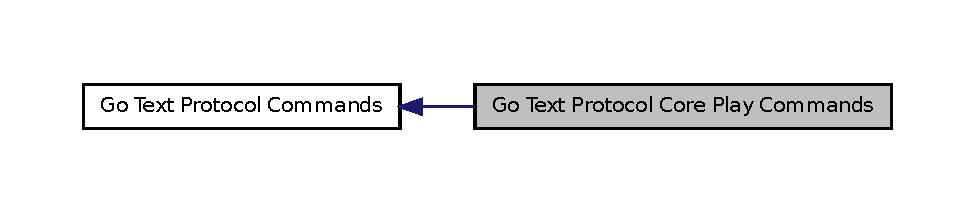
\includegraphics[width=400pt]{group___g_t_p___core___play___commands}
\end{center}
\end{figure}


\subsection*{Functions}
\begin{DoxyCompactItemize}
\item 
void \hyperlink{group___g_t_p___core___play___commands_ga16a060c01868977200be0b381b03c6f9}{gtp\_\-play} (int gtp\_\-argc, char gtp\_\-argv\mbox{[}$\,$\mbox{]}\mbox{[}MAX\_\-TOKEN\_\-LENGTH\mbox{]})
\begin{DoxyCompactList}\small\item\em Description missing! \item\end{DoxyCompactList}\end{DoxyCompactItemize}


\subsection{Function Documentation}
\hypertarget{group___g_t_p___core___play___commands_ga16a060c01868977200be0b381b03c6f9}{
\index{GTP\_\-Core\_\-Play\_\-Commands@{GTP\_\-Core\_\-Play\_\-Commands}!gtp\_\-play@{gtp\_\-play}}
\index{gtp\_\-play@{gtp\_\-play}!GTP_Core_Play_Commands@{GTP\_\-Core\_\-Play\_\-Commands}}
\subsubsection[{gtp\_\-play}]{\setlength{\rightskip}{0pt plus 5cm}void gtp\_\-play (
\begin{DoxyParamCaption}
\item[{int}]{ gtp\_\-argc, }
\item[{char}]{ gtp\_\-argv\mbox{[}$\,$\mbox{]}\mbox{[}MAX\_\-TOKEN\_\-LENGTH\mbox{]}}
\end{DoxyParamCaption}
)}}
\label{group___g_t_p___core___play___commands_ga16a060c01868977200be0b381b03c6f9}


Description missing! 

\hyperlink{group___g_t_p___core___play___commands_ga16a060c01868977200be0b381b03c6f9}{gtp\_\-play()} Description missing!

\begin{Desc}
\item[\hyperlink{todo__todo000004}{Todo}]Description is missing!\end{Desc}



\begin{DoxyParams}{Parameters}
\item[\mbox{\tt[in]} {\em gtp\_\-argc}]Number of arguments of GTP command \item[\mbox{\tt[in]} {\em gtp\_\-argv}]Array of all arguments for GTP command \end{DoxyParams}
\begin{DoxyReturn}{Returns}
nothing 
\end{DoxyReturn}
\begin{DoxySeeAlso}{See also}
Go Text Protokol version 2, 6.3.3 Core Play Commands 
\end{DoxySeeAlso}


\begin{Desc}
\item[\hyperlink{todo__todo000005}{Todo}]Remove captured stones here ... \end{Desc}
\begin{Desc}
\item[\hyperlink{todo__todo000006}{Todo}]Update move history ... \end{Desc}




Definition at line 545 of file run\_\-program.c.




\begin{DoxyCode}
{
    int color;
    int i, j;

    // Check if first argument is black or white:
    str_toupper( gtp_argv[0] );
    if ( strcmp( gtp_argv[0], "B" ) == 0 || strcmp( gtp_argv[0], "BLACK" ) == 0 )
       {
        color = BLACK;
    }
    else if ( strcmp( gtp_argv[0], "W" ) == 0 || strcmp( gtp_argv[0], "WHITE" ) =
      = 0 ) {
        color = WHITE;
    }
    else {
        set_output_error();
        add_output("invalid color");
        return;
    }

    // Check vertex if first coordinate is valid:
    i = (int) toupper( gtp_argv[1][0] ) - 65;
    if ( i > 8 ) {
        i--;
    }
    if ( i < 0 || i >= get_board_size() ) {
        set_output_error();
        add_output("invalid coordinate");
        return;
    }

    // Check if second coordinate is valid:
    gtp_argv[1][0] = ' ';
    j = (int) atoi( gtp_argv[1] );
    j--;
    if ( j < 0 || j >= get_board_size() ) {
        set_output_error();
        add_output("invalid coordinate");
        return;
    }

    set_vertex( color, i, j );


    return;
}
\end{DoxyCode}



\hypertarget{group___g_t_p___debug___commands}{
\section{Go Text Protocol Debug Commands}
\label{group___g_t_p___debug___commands}\index{Go Text Protocol Debug Commands@{Go Text Protocol Debug Commands}}
}


Collaboration diagram for Go Text Protocol Debug Commands:\nopagebreak
\begin{figure}[H]
\begin{center}
\leavevmode
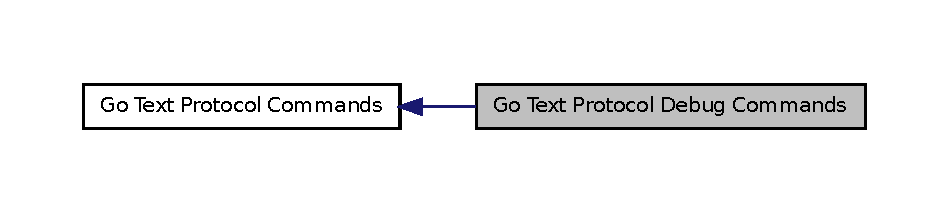
\includegraphics[width=400pt]{group___g_t_p___debug___commands}
\end{center}
\end{figure}


\subsection*{Functions}
\begin{DoxyCompactItemize}
\item 
void \hyperlink{group___g_t_p___debug___commands_ga7c297f28150386dc85b1de08e6f8d456}{gtp\_\-showboard} (int gtp\_\-argc, char gtp\_\-argv\mbox{[}$\,$\mbox{]}\mbox{[}MAX\_\-TOKEN\_\-LENGTH\mbox{]})
\begin{DoxyCompactList}\small\item\em Shows a simple ASCII board. \item\end{DoxyCompactList}\end{DoxyCompactItemize}


\subsection{Function Documentation}
\hypertarget{group___g_t_p___debug___commands_ga7c297f28150386dc85b1de08e6f8d456}{
\index{GTP\_\-Debug\_\-Commands@{GTP\_\-Debug\_\-Commands}!gtp\_\-showboard@{gtp\_\-showboard}}
\index{gtp\_\-showboard@{gtp\_\-showboard}!GTP_Debug_Commands@{GTP\_\-Debug\_\-Commands}}
\subsubsection[{gtp\_\-showboard}]{\setlength{\rightskip}{0pt plus 5cm}void gtp\_\-showboard (
\begin{DoxyParamCaption}
\item[{int}]{ gtp\_\-argc, }
\item[{char}]{ gtp\_\-argv\mbox{[}$\,$\mbox{]}\mbox{[}MAX\_\-TOKEN\_\-LENGTH\mbox{]}}
\end{DoxyParamCaption}
)}}
\label{group___g_t_p___debug___commands_ga7c297f28150386dc85b1de08e6f8d456}


Shows a simple ASCII board. 

\begin{Desc}
\item[\hyperlink{todo__todo000003}{Todo}]These functions have to be implemmted: gtp\_\-genmove, gtp\_\-undo.
\begin{DoxyItemize}
\item void gtp\_\-genmove( int argc, char argv\mbox{[}\mbox{]}\mbox{[}MAX\_\-TOKEN\_\-LENGTH\mbox{]} );
\item void gtp\_\-undo( int argc, char argv\mbox{[}\mbox{]}\mbox{[}MAX\_\-TOKEN\_\-LENGTH\mbox{]} ); 
\end{DoxyItemize}\end{Desc}


\hyperlink{group___g_t_p___debug___commands_ga7c297f28150386dc85b1de08e6f8d456}{gtp\_\-showboard()} gets a string representation of the board and sends it to the board\_\-output variable, so it can then be printed.


\begin{DoxyParams}{Parameters}
\item[\mbox{\tt[in]} {\em gtp\_\-argc}]Number of arguments of GTP command \item[\mbox{\tt[in]} {\em gtp\_\-argv}]Array of all arguments for GTP command \end{DoxyParams}
\begin{DoxyReturn}{Returns}
nothing 
\end{DoxyReturn}
\begin{DoxySeeAlso}{See also}
Go Text Protokol version 2, 6.3.6 Debug Commands 
\end{DoxySeeAlso}


Definition at line 609 of file run\_\-program.c.




\begin{DoxyCode}
{
    char board_output[MAX_OUTPUT_LENGTH];

    get_board_as_string(board_output);
    add_output(board_output);

    return;
}
\end{DoxyCode}



\chapter{Data Structure Documentation}
\hypertarget{structcommand}{
\section{command Struct Reference}
\label{structcommand}\index{command@{command}}
}


{\ttfamily \#include $<$io.h$>$}

\subsection*{Data Fields}
\begin{DoxyCompactItemize}
\item 
int \hyperlink{structcommand_a7441ef0865bcb3db9b8064dd7375c1ea}{id}
\item 
char \hyperlink{structcommand_ac0b9897814a00cff684163a205d092b4}{name} \mbox{[}MAX\_\-TOKEN\_\-LENGTH\mbox{]}
\item 
char \hyperlink{structcommand_aad4787c27c68e4bb76cfca730a8db9e0}{gtp\_\-argv} \mbox{[}MAX\_\-TOKEN\_\-COUNT+1\mbox{]}\mbox{[}MAX\_\-TOKEN\_\-LENGTH\mbox{]}
\item 
int \hyperlink{structcommand_a27d38bda7ae19f88a83100379e972da9}{gtp\_\-argc}
\end{DoxyCompactItemize}


\subsection{Detailed Description}


Definition at line 9 of file io.h.



\subsection{Field Documentation}
\hypertarget{structcommand_a27d38bda7ae19f88a83100379e972da9}{
\index{command@{command}!gtp\_\-argc@{gtp\_\-argc}}
\index{gtp\_\-argc@{gtp\_\-argc}!command@{command}}
\subsubsection[{gtp\_\-argc}]{\setlength{\rightskip}{0pt plus 5cm}int {\bf gtp\_\-argc}}}
\label{structcommand_a27d38bda7ae19f88a83100379e972da9}


Definition at line 13 of file io.h.

\hypertarget{structcommand_aad4787c27c68e4bb76cfca730a8db9e0}{
\index{command@{command}!gtp\_\-argv@{gtp\_\-argv}}
\index{gtp\_\-argv@{gtp\_\-argv}!command@{command}}
\subsubsection[{gtp\_\-argv}]{\setlength{\rightskip}{0pt plus 5cm}char {\bf gtp\_\-argv}\mbox{[}MAX\_\-TOKEN\_\-COUNT+1\mbox{]}\mbox{[}MAX\_\-TOKEN\_\-LENGTH\mbox{]}}}
\label{structcommand_aad4787c27c68e4bb76cfca730a8db9e0}


Definition at line 12 of file io.h.

\hypertarget{structcommand_a7441ef0865bcb3db9b8064dd7375c1ea}{
\index{command@{command}!id@{id}}
\index{id@{id}!command@{command}}
\subsubsection[{id}]{\setlength{\rightskip}{0pt plus 5cm}int {\bf id}}}
\label{structcommand_a7441ef0865bcb3db9b8064dd7375c1ea}


Definition at line 10 of file io.h.

\hypertarget{structcommand_ac0b9897814a00cff684163a205d092b4}{
\index{command@{command}!name@{name}}
\index{name@{name}!command@{command}}
\subsubsection[{name}]{\setlength{\rightskip}{0pt plus 5cm}char {\bf name}\mbox{[}MAX\_\-TOKEN\_\-LENGTH\mbox{]}}}
\label{structcommand_ac0b9897814a00cff684163a205d092b4}


Definition at line 11 of file io.h.



The documentation for this struct was generated from the following file:\begin{DoxyCompactItemize}
\item 
src/\hyperlink{io_8h}{io.h}\end{DoxyCompactItemize}

\hypertarget{structcommand__func}{
\section{command\_\-func Struct Reference}
\label{structcommand__func}\index{command\_\-func@{command\_\-func}}
}


Connects one given command name with proper function pointer.  


\subsection*{Data Fields}
\begin{DoxyCompactItemize}
\item 
char \hyperlink{structcommand__func_abd43b5b64c261a18978a168e6c3db44d}{command} \mbox{[}MAX\_\-TOKEN\_\-LENGTH\mbox{]}
\begin{DoxyCompactList}\small\item\em Sets the name of the GTP command. \item\end{DoxyCompactList}\item 
void($\ast$ \hyperlink{structcommand__func_a6922e0c4b7e05be375cde200d2788c89}{function} )()
\begin{DoxyCompactList}\small\item\em Sets the pointer to the function for GTP command. \item\end{DoxyCompactList}\end{DoxyCompactItemize}


\subsection{Detailed Description}
Connects one given command name with proper function pointer. \begin{Desc}
\item[\hyperlink{todo__todo000002}{Todo}]Check if function declaration needs parameters! \end{Desc}


Definition at line 25 of file run\_\-program.c.



\subsection{Field Documentation}
\hypertarget{structcommand__func_abd43b5b64c261a18978a168e6c3db44d}{
\index{command\_\-func@{command\_\-func}!command@{command}}
\index{command@{command}!command_func@{command\_\-func}}
\subsubsection[{command}]{\setlength{\rightskip}{0pt plus 5cm}char {\bf command}\mbox{[}MAX\_\-TOKEN\_\-LENGTH\mbox{]}}}
\label{structcommand__func_abd43b5b64c261a18978a168e6c3db44d}


Sets the name of the GTP command. 



Definition at line 26 of file run\_\-program.c.

\hypertarget{structcommand__func_a6922e0c4b7e05be375cde200d2788c89}{
\index{command\_\-func@{command\_\-func}!function@{function}}
\index{function@{function}!command_func@{command\_\-func}}
\subsubsection[{function}]{\setlength{\rightskip}{0pt plus 5cm}void($\ast$ {\bf function})()}}
\label{structcommand__func_a6922e0c4b7e05be375cde200d2788c89}


Sets the pointer to the function for GTP command. 



Definition at line 27 of file run\_\-program.c.



The documentation for this struct was generated from the following file:\begin{DoxyCompactItemize}
\item 
src/\hyperlink{run__program_8c}{run\_\-program.c}\end{DoxyCompactItemize}

\chapter{File Documentation}
\hypertarget{board_8c}{
\section{src/board.c File Reference}
\label{board_8c}\index{src/board.c@{src/board.c}}
}
{\ttfamily \#include $<$stdlib.h$>$}\par
{\ttfamily \#include $<$stdio.h$>$}\par
{\ttfamily \#include $<$string.h$>$}\par
{\ttfamily \#include $<$stdbool.h$>$}\par
{\ttfamily \#include \char`\"{}global\_\-const.h\char`\"{}}\par
{\ttfamily \#include \char`\"{}board.h\char`\"{}}\par
Include dependency graph for board.c:\nopagebreak
\begin{figure}[H]
\begin{center}
\leavevmode
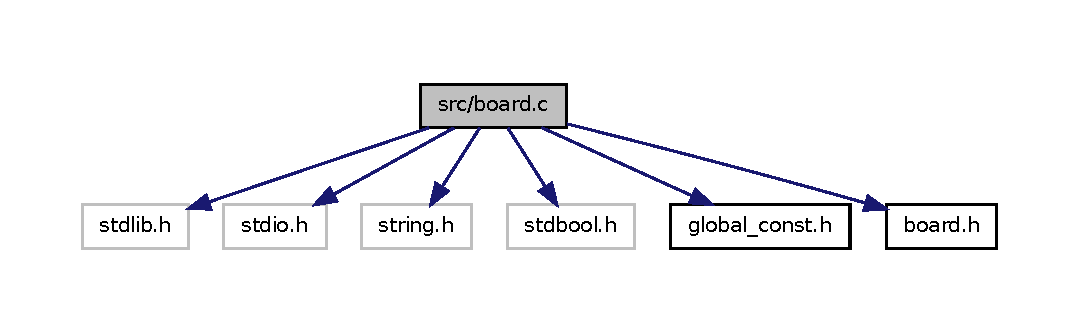
\includegraphics[width=400pt]{board_8c__incl}
\end{center}
\end{figure}
\subsection*{Functions}
\begin{DoxyCompactItemize}
\item 
void \hyperlink{board_8c_a638155d3ce2a053895a9c626e480b4f6}{get\_\-label\_\-x} (int i, char x\mbox{[}$\,$\mbox{]})
\item 
void \hyperlink{board_8c_acdcf055eb485579afb015abf054f66d8}{get\_\-label\_\-y\_\-left} (int i, char x\mbox{[}$\,$\mbox{]})
\item 
void \hyperlink{board_8c_a1d09579c09a783962a8d29005552e5c1}{get\_\-label\_\-y\_\-right} (int j, char y\mbox{[}$\,$\mbox{]})
\item 
bool \hyperlink{board_8c_a16e95d81990e946e33bf1b2a9d75bc80}{is\_\-hoshi} (int i, int j)
\item 
void \hyperlink{board_8c_ac70f31e9f413033ba999d4eccb459cb5}{init\_\-board} (int wanted\_\-board\_\-size)
\begin{DoxyCompactList}\small\item\em Allocates memory for all board data structures. \item\end{DoxyCompactList}\item 
void \hyperlink{board_8c_a96dcf44b26f99e5b5f3ebfaa31bf7162}{free\_\-board} (void)
\item 
void \hyperlink{board_8c_ac82f164590b043f9ef44c37ecca4acb0}{get\_\-board\_\-as\_\-string} (char board\_\-output\mbox{[}$\,$\mbox{]})
\item 
int \hyperlink{board_8c_aa870bb6580c6bce8bb91da8682f8bbf7}{get\_\-board\_\-size} (void)
\item 
void \hyperlink{board_8c_ad0341838fa4fa4d4279c5f050cf96feb}{set\_\-vertex} (int color, int i, int j)
\end{DoxyCompactItemize}
\subsection*{Variables}
\begin{DoxyCompactItemize}
\item 
int $\ast$$\ast$ \hyperlink{board_8c_af47ada0fcdb12bc1fe48c1eaef29e1a3}{board}
\item 
bool $\ast$$\ast$ \hyperlink{board_8c_ae5779438e79e100a9d0e3ec5270b127e}{hoshi}
\item 
int \hyperlink{board_8c_a1220b475fc44e0a5dcb883e811d1834f}{board\_\-size} = 0
\end{DoxyCompactItemize}


\subsection{Function Documentation}
\hypertarget{board_8c_a96dcf44b26f99e5b5f3ebfaa31bf7162}{
\index{board.c@{board.c}!free\_\-board@{free\_\-board}}
\index{free\_\-board@{free\_\-board}!board.c@{board.c}}
\subsubsection[{free\_\-board}]{\setlength{\rightskip}{0pt plus 5cm}void free\_\-board (
\begin{DoxyParamCaption}
\item[{void}]{}
\end{DoxyParamCaption}
)}}
\label{board_8c_a96dcf44b26f99e5b5f3ebfaa31bf7162}


Definition at line 100 of file board.c.




\begin{DoxyCode}
                      {
    int i;

    for ( i = 0; i < board_size; i++ ) {
        free(board[i]);
        free(hoshi[i]);
    }
    free(board);
    free(hoshi);

    return;
}
\end{DoxyCode}


\hypertarget{board_8c_ac82f164590b043f9ef44c37ecca4acb0}{
\index{board.c@{board.c}!get\_\-board\_\-as\_\-string@{get\_\-board\_\-as\_\-string}}
\index{get\_\-board\_\-as\_\-string@{get\_\-board\_\-as\_\-string}!board.c@{board.c}}
\subsubsection[{get\_\-board\_\-as\_\-string}]{\setlength{\rightskip}{0pt plus 5cm}void get\_\-board\_\-as\_\-string (
\begin{DoxyParamCaption}
\item[{char}]{ board\_\-output\mbox{[}$\,$\mbox{]}}
\end{DoxyParamCaption}
)}}
\label{board_8c_ac82f164590b043f9ef44c37ecca4acb0}


Definition at line 122 of file board.c.




\begin{DoxyCode}
                                                {
    int i; // Index for x-axis
    int j; // Index for y-axis
    char x[3];      // Label for x-axis
    char y[2];      // Label for y-axis

    board_output[0] = '\0';
    strcat( board_output, "\n" );

    /* Print uppercase letters above the board */
    strcat( board_output, "   " );
    for ( i = 0; i < board_size; i++ ) {
        get_label_x( i, x );
        strcat( board_output, " " );
        strcat( board_output, x );
    }
    strcat( board_output, "\n" );

    for ( j = board_size - 1; j >= 0; j-- ) {

        /* Print numbers left of board */
        get_label_y_left( j, y );
        strcat( board_output, " " );
        strcat( board_output, y );

        /* Print board fields */
        for ( i = 0; i < board_size; i++ ) {
            strcat( board_output, " " );
            switch ( board[i][j] ) {
                case WHITE:
                    strcat( board_output, WHITE_STONE );
                    break;
                case BLACK:
                    strcat( board_output, BLACK_STONE );
                    break;
                case EMPTY:
                    switch ( is_hoshi( i, j ) ) {
                        case true:
                            strcat( board_output, FIELD_HOSHI );
                            break;
                        case false:
                            strcat( board_output, FIELD_EMPTY );
                            break;
                    }
                    break;
            }
        }

        /* Print numbers right of board */
        get_label_y_right( j, y );
        strcat( board_output,  " " );
        strcat( board_output,    y );
        strcat( board_output, "\n" );
    }

    /* Print uppercase letters below board */
    strcat( board_output, "   " );
    for ( i = 0; i < board_size; i++ ) {
        get_label_x( i, x );
        strcat( board_output, " " );
        strcat( board_output, x );
    }

    return;
}
\end{DoxyCode}


\hypertarget{board_8c_aa870bb6580c6bce8bb91da8682f8bbf7}{
\index{board.c@{board.c}!get\_\-board\_\-size@{get\_\-board\_\-size}}
\index{get\_\-board\_\-size@{get\_\-board\_\-size}!board.c@{board.c}}
\subsubsection[{get\_\-board\_\-size}]{\setlength{\rightskip}{0pt plus 5cm}int get\_\-board\_\-size (
\begin{DoxyParamCaption}
\item[{void}]{}
\end{DoxyParamCaption}
)}}
\label{board_8c_aa870bb6580c6bce8bb91da8682f8bbf7}


Definition at line 234 of file board.c.




\begin{DoxyCode}
                         {

    return board_size;
}
\end{DoxyCode}


\hypertarget{board_8c_a638155d3ce2a053895a9c626e480b4f6}{
\index{board.c@{board.c}!get\_\-label\_\-x@{get\_\-label\_\-x}}
\index{get\_\-label\_\-x@{get\_\-label\_\-x}!board.c@{board.c}}
\subsubsection[{get\_\-label\_\-x}]{\setlength{\rightskip}{0pt plus 5cm}void get\_\-label\_\-x (
\begin{DoxyParamCaption}
\item[{int}]{ i, }
\item[{char}]{ x\mbox{[}$\,$\mbox{]}}
\end{DoxyParamCaption}
)}}
\label{board_8c_a638155d3ce2a053895a9c626e480b4f6}


Definition at line 188 of file board.c.




\begin{DoxyCode}
                                    {

    if ( i >= 8 ) {
        i++;
    }
    i += 65;
    x[0] = (char) i;
    x[1] = '\0';

    return;
}
\end{DoxyCode}


\hypertarget{board_8c_acdcf055eb485579afb015abf054f66d8}{
\index{board.c@{board.c}!get\_\-label\_\-y\_\-left@{get\_\-label\_\-y\_\-left}}
\index{get\_\-label\_\-y\_\-left@{get\_\-label\_\-y\_\-left}!board.c@{board.c}}
\subsubsection[{get\_\-label\_\-y\_\-left}]{\setlength{\rightskip}{0pt plus 5cm}void get\_\-label\_\-y\_\-left (
\begin{DoxyParamCaption}
\item[{int}]{ i, }
\item[{char}]{ x\mbox{[}$\,$\mbox{]}}
\end{DoxyParamCaption}
)}}
\label{board_8c_acdcf055eb485579afb015abf054f66d8}


Definition at line 200 of file board.c.




\begin{DoxyCode}
                                         {

    j++;

    y[0] = (char)(int)( j / 10 + 48 );
    y[1] = (char)( j % 10 + 48 );
    y[2] = '\0';
    if ( y[0] == '0' ) {
        y[0] = ' ';
    }

    return;
}
\end{DoxyCode}


\hypertarget{board_8c_a1d09579c09a783962a8d29005552e5c1}{
\index{board.c@{board.c}!get\_\-label\_\-y\_\-right@{get\_\-label\_\-y\_\-right}}
\index{get\_\-label\_\-y\_\-right@{get\_\-label\_\-y\_\-right}!board.c@{board.c}}
\subsubsection[{get\_\-label\_\-y\_\-right}]{\setlength{\rightskip}{0pt plus 5cm}void get\_\-label\_\-y\_\-right (
\begin{DoxyParamCaption}
\item[{int}]{ j, }
\item[{char}]{ y\mbox{[}$\,$\mbox{]}}
\end{DoxyParamCaption}
)}}
\label{board_8c_a1d09579c09a783962a8d29005552e5c1}


Definition at line 214 of file board.c.




\begin{DoxyCode}
                                          {

    j++;

    y[0] = (char)(int)( j / 10 + 48 );
    y[1] = (char)( j % 10 + 48 );
    y[2] = '\0';
    if ( y[0] == '0' ) {
        y[0] = y[1];
        y[1] = '\0';
    }

    return;
}
\end{DoxyCode}


\hypertarget{board_8c_ac70f31e9f413033ba999d4eccb459cb5}{
\index{board.c@{board.c}!init\_\-board@{init\_\-board}}
\index{init\_\-board@{init\_\-board}!board.c@{board.c}}
\subsubsection[{init\_\-board}]{\setlength{\rightskip}{0pt plus 5cm}void init\_\-board (
\begin{DoxyParamCaption}
\item[{int}]{ wanted\_\-board\_\-size}
\end{DoxyParamCaption}
)}}
\label{board_8c_ac70f31e9f413033ba999d4eccb459cb5}


Allocates memory for all board data structures. 

Allocates memory for the data structures board and hoshi. Its sets the board fields to EMPTY and sets the correct hoshi points depending on board size.


\begin{DoxyParams}{Parameters}
\item[\mbox{\tt[in]} {\em wanted\_\-board\_\-size}]Integer of intended board size \end{DoxyParams}
\begin{DoxyReturn}{Returns}
nothing 
\end{DoxyReturn}
\begin{DoxySeeAlso}{See also}
\mbox{[}n/a\mbox{]}
\end{DoxySeeAlso}
\begin{Desc}
\item[\hyperlink{todo__todo000001}{Todo}]A size check has to be implemented probably. \end{Desc}


Definition at line 33 of file board.c.




\begin{DoxyCode}
{
    int i, j;

    board_size = wanted_board_size;

    board = malloc( board_size * sizeof(int *) );
    hoshi = malloc( board_size * sizeof(bool *) );
    if ( board == NULL || hoshi == NULL ) {
        fprintf( stderr, "Failed to malloc memory");
        exit(EXIT_FAILURE);
    }

    for ( i = 0; i < board_size; i++ ) {
        board[i] = malloc( board_size * sizeof(int) );
        hoshi[i] = malloc( board_size * sizeof(bool) );
        if ( board[i] == NULL || hoshi[i] == NULL ) {
            fprintf( stderr, "Failed to malloc memory");
            exit(EXIT_FAILURE);
        }

        for ( j = 0; j < board_size; j++ ) {
            board[i][j] = EMPTY;
            hoshi[i][j] = false;
        }
    }

    switch (board_size) {
        case 19:
            hoshi[3][3]   = true;
            hoshi[3][9]   = true;
            hoshi[3][15]  = true;
            hoshi[9][3]   = true;
            hoshi[9][9]   = true;
            hoshi[9][15]  = true;
            hoshi[15][3]  = true;
            hoshi[15][9]  = true;
            hoshi[15][15] = true;
            break;
        case 13:
            hoshi[3][3] = true;
            hoshi[3][9] = true;
            hoshi[9][3] = true;
            hoshi[9][9] = true;
            hoshi[6][6] = true;
            break;
        case 9:
            hoshi[2][2] = true;
            hoshi[2][6] = true;
            hoshi[6][2] = true;
            hoshi[6][6] = true;
            hoshi[4][4] = true;
            break;
    }

    return;
}
\end{DoxyCode}


\hypertarget{board_8c_a16e95d81990e946e33bf1b2a9d75bc80}{
\index{board.c@{board.c}!is\_\-hoshi@{is\_\-hoshi}}
\index{is\_\-hoshi@{is\_\-hoshi}!board.c@{board.c}}
\subsubsection[{is\_\-hoshi}]{\setlength{\rightskip}{0pt plus 5cm}bool is\_\-hoshi (
\begin{DoxyParamCaption}
\item[{int}]{ i, }
\item[{int}]{ j}
\end{DoxyParamCaption}
)}}
\label{board_8c_a16e95d81990e946e33bf1b2a9d75bc80}


Definition at line 229 of file board.c.




\begin{DoxyCode}
                              {

    return hoshi[i][j];
}
\end{DoxyCode}


\hypertarget{board_8c_ad0341838fa4fa4d4279c5f050cf96feb}{
\index{board.c@{board.c}!set\_\-vertex@{set\_\-vertex}}
\index{set\_\-vertex@{set\_\-vertex}!board.c@{board.c}}
\subsubsection[{set\_\-vertex}]{\setlength{\rightskip}{0pt plus 5cm}void set\_\-vertex (
\begin{DoxyParamCaption}
\item[{int}]{ color, }
\item[{int}]{ i, }
\item[{int}]{ j}
\end{DoxyParamCaption}
)}}
\label{board_8c_ad0341838fa4fa4d4279c5f050cf96feb}


Definition at line 239 of file board.c.




\begin{DoxyCode}
                                           {

    board[i][j] = color;

    return;
}
\end{DoxyCode}




\subsection{Variable Documentation}
\hypertarget{board_8c_af47ada0fcdb12bc1fe48c1eaef29e1a3}{
\index{board.c@{board.c}!board@{board}}
\index{board@{board}!board.c@{board.c}}
\subsubsection[{board}]{\setlength{\rightskip}{0pt plus 5cm}int$\ast$$\ast$ {\bf board}}}
\label{board_8c_af47ada0fcdb12bc1fe48c1eaef29e1a3}


Definition at line 9 of file board.c.

\hypertarget{board_8c_a1220b475fc44e0a5dcb883e811d1834f}{
\index{board.c@{board.c}!board\_\-size@{board\_\-size}}
\index{board\_\-size@{board\_\-size}!board.c@{board.c}}
\subsubsection[{board\_\-size}]{\setlength{\rightskip}{0pt plus 5cm}int {\bf board\_\-size} = 0}}
\label{board_8c_a1220b475fc44e0a5dcb883e811d1834f}


Definition at line 12 of file board.c.

\hypertarget{board_8c_ae5779438e79e100a9d0e3ec5270b127e}{
\index{board.c@{board.c}!hoshi@{hoshi}}
\index{hoshi@{hoshi}!board.c@{board.c}}
\subsubsection[{hoshi}]{\setlength{\rightskip}{0pt plus 5cm}bool$\ast$$\ast$ {\bf hoshi}}}
\label{board_8c_ae5779438e79e100a9d0e3ec5270b127e}


Definition at line 10 of file board.c.


\hypertarget{board_8h}{
\section{src/board.h File Reference}
\label{board_8h}\index{src/board.h@{src/board.h}}
}
This graph shows which files directly or indirectly include this file:\nopagebreak
\begin{figure}[H]
\begin{center}
\leavevmode
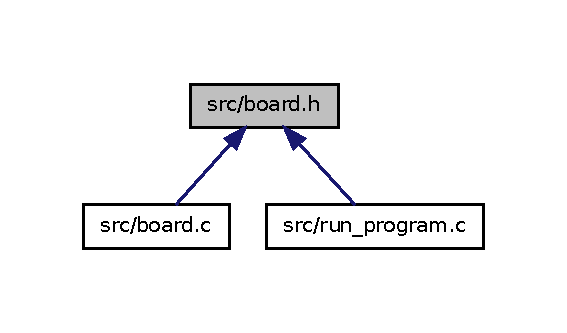
\includegraphics[width=272pt]{board_8h__dep__incl}
\end{center}
\end{figure}
\subsection*{Functions}
\begin{DoxyCompactItemize}
\item 
void \hyperlink{board_8h_ac70f31e9f413033ba999d4eccb459cb5}{init\_\-board} (int wanted\_\-board\_\-size)
\begin{DoxyCompactList}\small\item\em Allocates memory for all board data structures. \item\end{DoxyCompactList}\item 
void \hyperlink{board_8h_a96dcf44b26f99e5b5f3ebfaa31bf7162}{free\_\-board} (void)
\item 
void \hyperlink{board_8h_ac82f164590b043f9ef44c37ecca4acb0}{get\_\-board\_\-as\_\-string} (char board\_\-output\mbox{[}$\,$\mbox{]})
\item 
int \hyperlink{board_8h_aa870bb6580c6bce8bb91da8682f8bbf7}{get\_\-board\_\-size} (void)
\item 
void \hyperlink{board_8h_ad0341838fa4fa4d4279c5f050cf96feb}{set\_\-vertex} (int color, int i, int j)
\end{DoxyCompactItemize}


\subsection{Function Documentation}
\hypertarget{board_8h_a96dcf44b26f99e5b5f3ebfaa31bf7162}{
\index{board.h@{board.h}!free\_\-board@{free\_\-board}}
\index{free\_\-board@{free\_\-board}!board.h@{board.h}}
\subsubsection[{free\_\-board}]{\setlength{\rightskip}{0pt plus 5cm}void free\_\-board (
\begin{DoxyParamCaption}
\item[{void}]{}
\end{DoxyParamCaption}
)}}
\label{board_8h_a96dcf44b26f99e5b5f3ebfaa31bf7162}


Definition at line 100 of file board.c.




\begin{DoxyCode}
                      {
    int i;

    for ( i = 0; i < board_size; i++ ) {
        free(board[i]);
        free(hoshi[i]);
    }
    free(board);
    free(hoshi);

    return;
}
\end{DoxyCode}


\hypertarget{board_8h_ac82f164590b043f9ef44c37ecca4acb0}{
\index{board.h@{board.h}!get\_\-board\_\-as\_\-string@{get\_\-board\_\-as\_\-string}}
\index{get\_\-board\_\-as\_\-string@{get\_\-board\_\-as\_\-string}!board.h@{board.h}}
\subsubsection[{get\_\-board\_\-as\_\-string}]{\setlength{\rightskip}{0pt plus 5cm}void get\_\-board\_\-as\_\-string (
\begin{DoxyParamCaption}
\item[{char}]{ board\_\-output\mbox{[}$\,$\mbox{]}}
\end{DoxyParamCaption}
)}}
\label{board_8h_ac82f164590b043f9ef44c37ecca4acb0}


Definition at line 122 of file board.c.




\begin{DoxyCode}
                                                {
    int i; // Index for x-axis
    int j; // Index for y-axis
    char x[3];      // Label for x-axis
    char y[2];      // Label for y-axis

    board_output[0] = '\0';
    strcat( board_output, "\n" );

    /* Print uppercase letters above the board */
    strcat( board_output, "   " );
    for ( i = 0; i < board_size; i++ ) {
        get_label_x( i, x );
        strcat( board_output, " " );
        strcat( board_output, x );
    }
    strcat( board_output, "\n" );

    for ( j = board_size - 1; j >= 0; j-- ) {

        /* Print numbers left of board */
        get_label_y_left( j, y );
        strcat( board_output, " " );
        strcat( board_output, y );

        /* Print board fields */
        for ( i = 0; i < board_size; i++ ) {
            strcat( board_output, " " );
            switch ( board[i][j] ) {
                case WHITE:
                    strcat( board_output, WHITE_STONE );
                    break;
                case BLACK:
                    strcat( board_output, BLACK_STONE );
                    break;
                case EMPTY:
                    switch ( is_hoshi( i, j ) ) {
                        case true:
                            strcat( board_output, FIELD_HOSHI );
                            break;
                        case false:
                            strcat( board_output, FIELD_EMPTY );
                            break;
                    }
                    break;
            }
        }

        /* Print numbers right of board */
        get_label_y_right( j, y );
        strcat( board_output,  " " );
        strcat( board_output,    y );
        strcat( board_output, "\n" );
    }

    /* Print uppercase letters below board */
    strcat( board_output, "   " );
    for ( i = 0; i < board_size; i++ ) {
        get_label_x( i, x );
        strcat( board_output, " " );
        strcat( board_output, x );
    }

    return;
}
\end{DoxyCode}


\hypertarget{board_8h_aa870bb6580c6bce8bb91da8682f8bbf7}{
\index{board.h@{board.h}!get\_\-board\_\-size@{get\_\-board\_\-size}}
\index{get\_\-board\_\-size@{get\_\-board\_\-size}!board.h@{board.h}}
\subsubsection[{get\_\-board\_\-size}]{\setlength{\rightskip}{0pt plus 5cm}int get\_\-board\_\-size (
\begin{DoxyParamCaption}
\item[{void}]{}
\end{DoxyParamCaption}
)}}
\label{board_8h_aa870bb6580c6bce8bb91da8682f8bbf7}


Definition at line 234 of file board.c.




\begin{DoxyCode}
                         {

    return board_size;
}
\end{DoxyCode}


\hypertarget{board_8h_ac70f31e9f413033ba999d4eccb459cb5}{
\index{board.h@{board.h}!init\_\-board@{init\_\-board}}
\index{init\_\-board@{init\_\-board}!board.h@{board.h}}
\subsubsection[{init\_\-board}]{\setlength{\rightskip}{0pt plus 5cm}void init\_\-board (
\begin{DoxyParamCaption}
\item[{int}]{ wanted\_\-board\_\-size}
\end{DoxyParamCaption}
)}}
\label{board_8h_ac70f31e9f413033ba999d4eccb459cb5}


Allocates memory for all board data structures. 

Allocates memory for the data structures board and hoshi. Its sets the board fields to EMPTY and sets the correct hoshi points depending on board size.


\begin{DoxyParams}{Parameters}
\item[\mbox{\tt[in]} {\em wanted\_\-board\_\-size}]Integer of intended board size \end{DoxyParams}
\begin{DoxyReturn}{Returns}
nothing 
\end{DoxyReturn}
\begin{DoxySeeAlso}{See also}
\mbox{[}n/a\mbox{]}
\end{DoxySeeAlso}
\begin{Desc}
\item[\hyperlink{todo__todo000001}{Todo}]A size check has to be implemented probably. \end{Desc}


Definition at line 33 of file board.c.




\begin{DoxyCode}
{
    int i, j;

    board_size = wanted_board_size;

    board = malloc( board_size * sizeof(int *) );
    hoshi = malloc( board_size * sizeof(bool *) );
    if ( board == NULL || hoshi == NULL ) {
        fprintf( stderr, "Failed to malloc memory");
        exit(EXIT_FAILURE);
    }

    for ( i = 0; i < board_size; i++ ) {
        board[i] = malloc( board_size * sizeof(int) );
        hoshi[i] = malloc( board_size * sizeof(bool) );
        if ( board[i] == NULL || hoshi[i] == NULL ) {
            fprintf( stderr, "Failed to malloc memory");
            exit(EXIT_FAILURE);
        }

        for ( j = 0; j < board_size; j++ ) {
            board[i][j] = EMPTY;
            hoshi[i][j] = false;
        }
    }

    switch (board_size) {
        case 19:
            hoshi[3][3]   = true;
            hoshi[3][9]   = true;
            hoshi[3][15]  = true;
            hoshi[9][3]   = true;
            hoshi[9][9]   = true;
            hoshi[9][15]  = true;
            hoshi[15][3]  = true;
            hoshi[15][9]  = true;
            hoshi[15][15] = true;
            break;
        case 13:
            hoshi[3][3] = true;
            hoshi[3][9] = true;
            hoshi[9][3] = true;
            hoshi[9][9] = true;
            hoshi[6][6] = true;
            break;
        case 9:
            hoshi[2][2] = true;
            hoshi[2][6] = true;
            hoshi[6][2] = true;
            hoshi[6][6] = true;
            hoshi[4][4] = true;
            break;
    }

    return;
}
\end{DoxyCode}


\hypertarget{board_8h_ad0341838fa4fa4d4279c5f050cf96feb}{
\index{board.h@{board.h}!set\_\-vertex@{set\_\-vertex}}
\index{set\_\-vertex@{set\_\-vertex}!board.h@{board.h}}
\subsubsection[{set\_\-vertex}]{\setlength{\rightskip}{0pt plus 5cm}void set\_\-vertex (
\begin{DoxyParamCaption}
\item[{int}]{ color, }
\item[{int}]{ i, }
\item[{int}]{ j}
\end{DoxyParamCaption}
)}}
\label{board_8h_ad0341838fa4fa4d4279c5f050cf96feb}


Definition at line 239 of file board.c.




\begin{DoxyCode}
                                           {

    board[i][j] = color;

    return;
}
\end{DoxyCode}



\hypertarget{global__const_8h}{
\section{src/global\_\-const.h File Reference}
\label{global__const_8h}\index{src/global\_\-const.h@{src/global\_\-const.h}}
}
This graph shows which files directly or indirectly include this file:\nopagebreak
\begin{figure}[H]
\begin{center}
\leavevmode
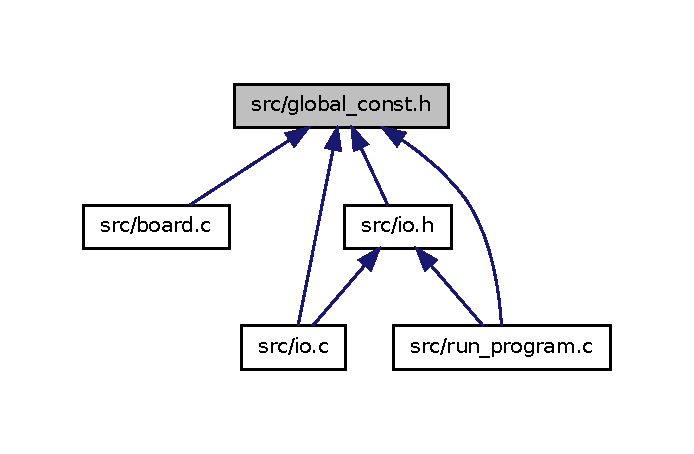
\includegraphics[width=333pt]{global__const_8h__dep__incl}
\end{center}
\end{figure}
\subsection*{Defines}
\begin{DoxyCompactItemize}
\item 
\#define \hyperlink{global__const_8h_a3b6a35b8be8405a9db72cc5dea97954b}{PROGRAM\_\-NAME}~\char`\"{}haigo\char`\"{}
\begin{DoxyCompactList}\small\item\em Defines the name of the program. \item\end{DoxyCompactList}\item 
\#define \hyperlink{global__const_8h_a2f10abd650e471fae2d7e8c63d41206a}{PROGRAM\_\-VERSION}~\char`\"{}0.1\char`\"{}
\begin{DoxyCompactList}\small\item\em Defines the current version of the program. \item\end{DoxyCompactList}\item 
\#define \hyperlink{global__const_8h_a36abee9957026d2840f9a0a47d4f4ee6}{VALID\_\-OPTIONS}~\char`\"{}hv\char`\"{}
\begin{DoxyCompactList}\small\item\em Defines the valid command line options. \item\end{DoxyCompactList}\item 
\#define \hyperlink{global__const_8h_af9aea523c04ab5371a8893039d45bda7}{GTP\_\-VERSION}~\char`\"{}2\char`\"{}
\begin{DoxyCompactList}\small\item\em Defines the implemented version of the Go Text Protocol. \item\end{DoxyCompactList}\item 
\#define \hyperlink{global__const_8h_a6ba86e8818f2fd7667971e2872dc24b0}{MAX\_\-TOKEN\_\-LENGTH}~20
\begin{DoxyCompactList}\small\item\em Defines the maximum length of any given GTP token, either command or argument. \item\end{DoxyCompactList}\item 
\#define \hyperlink{global__const_8h_a8c2b776cce16ba8e6fff75b2c721b8ac}{MAX\_\-TOKEN\_\-COUNT}~10
\begin{DoxyCompactList}\small\item\em Defines the maximum number of given GTP tokens for any command plus arguments. \item\end{DoxyCompactList}\item 
\#define \hyperlink{global__const_8h_abe831c824f88924a860426a29707b269}{MAX\_\-OUTPUT\_\-LENGTH}~2048
\begin{DoxyCompactList}\small\item\em Sets the length of the GTP output buffer. \item\end{DoxyCompactList}\item 
\#define \hyperlink{global__const_8h_a2b7cf2a3641be7b89138615764d60ba3}{EMPTY}~0
\begin{DoxyCompactList}\small\item\em Constant for an empty field. \item\end{DoxyCompactList}\item 
\#define \hyperlink{global__const_8h_a7b3b25cba33b07c303f3060fe41887f6}{BLACK}~1
\begin{DoxyCompactList}\small\item\em Constant for black stone. \item\end{DoxyCompactList}\item 
\#define \hyperlink{global__const_8h_a87b537f5fa5c109d3c05c13d6b18f382}{WHITE}~-\/1
\begin{DoxyCompactList}\small\item\em Constant for white stone. \item\end{DoxyCompactList}\item 
\#define \hyperlink{global__const_8h_a88ab06f28cdd25210fbec72e9ea3ded4}{FIELD\_\-EMPTY}~\char`\"{}.\char`\"{}
\begin{DoxyCompactList}\small\item\em Defines the character which is shown for an empty field. \item\end{DoxyCompactList}\item 
\#define \hyperlink{global__const_8h_a3772ccd34675a41954d7de5ad084e432}{FIELD\_\-HOSHI}~\char`\"{}+\char`\"{}
\begin{DoxyCompactList}\small\item\em Defines the character which is shown for a star field. \item\end{DoxyCompactList}\item 
\#define \hyperlink{global__const_8h_a57f19414241d4970fa3ff164412afb2f}{WHITE\_\-STONE}~\char`\"{}0\char`\"{}
\begin{DoxyCompactList}\small\item\em Defines the character which is shown for a white stone. \item\end{DoxyCompactList}\item 
\#define \hyperlink{global__const_8h_a86afd23aa5695c0e4f938db48f810797}{BLACK\_\-STONE}~\char`\"{}X\char`\"{}
\begin{DoxyCompactList}\small\item\em Defines the character which is shown for a black stone. \item\end{DoxyCompactList}\item 
\#define \hyperlink{global__const_8h_aaec8d05d0e9a158a9e120cfb3858c867}{BOARD\_\-SIZE\_\-MIN}~2
\begin{DoxyCompactList}\small\item\em Defines the minimum board size which is accepted. \item\end{DoxyCompactList}\item 
\#define \hyperlink{global__const_8h_a668553103c8bb26f7bd5727eb5fdccf9}{BOARD\_\-SIZE\_\-MAX}~25
\begin{DoxyCompactList}\small\item\em Defines the maximum board size which is accepted. \item\end{DoxyCompactList}\item 
\#define \hyperlink{global__const_8h_acf9fdbe777d70427b1abbfac13c249d9}{BOARD\_\-SIZE\_\-DEFAULT}~19
\begin{DoxyCompactList}\small\item\em Defines the default board size. \item\end{DoxyCompactList}\end{DoxyCompactItemize}


\subsection{Define Documentation}
\hypertarget{global__const_8h_a7b3b25cba33b07c303f3060fe41887f6}{
\index{global\_\-const.h@{global\_\-const.h}!BLACK@{BLACK}}
\index{BLACK@{BLACK}!global_const.h@{global\_\-const.h}}
\subsubsection[{BLACK}]{\setlength{\rightskip}{0pt plus 5cm}\#define BLACK~1}}
\label{global__const_8h_a7b3b25cba33b07c303f3060fe41887f6}


Constant for black stone. 



Definition at line 25 of file global\_\-const.h.

\hypertarget{global__const_8h_a86afd23aa5695c0e4f938db48f810797}{
\index{global\_\-const.h@{global\_\-const.h}!BLACK\_\-STONE@{BLACK\_\-STONE}}
\index{BLACK\_\-STONE@{BLACK\_\-STONE}!global_const.h@{global\_\-const.h}}
\subsubsection[{BLACK\_\-STONE}]{\setlength{\rightskip}{0pt plus 5cm}\#define BLACK\_\-STONE~\char`\"{}X\char`\"{}}}
\label{global__const_8h_a86afd23aa5695c0e4f938db48f810797}


Defines the character which is shown for a black stone. 



Definition at line 36 of file global\_\-const.h.

\hypertarget{global__const_8h_acf9fdbe777d70427b1abbfac13c249d9}{
\index{global\_\-const.h@{global\_\-const.h}!BOARD\_\-SIZE\_\-DEFAULT@{BOARD\_\-SIZE\_\-DEFAULT}}
\index{BOARD\_\-SIZE\_\-DEFAULT@{BOARD\_\-SIZE\_\-DEFAULT}!global_const.h@{global\_\-const.h}}
\subsubsection[{BOARD\_\-SIZE\_\-DEFAULT}]{\setlength{\rightskip}{0pt plus 5cm}\#define BOARD\_\-SIZE\_\-DEFAULT~19}}
\label{global__const_8h_acf9fdbe777d70427b1abbfac13c249d9}


Defines the default board size. 



Definition at line 43 of file global\_\-const.h.

\hypertarget{global__const_8h_a668553103c8bb26f7bd5727eb5fdccf9}{
\index{global\_\-const.h@{global\_\-const.h}!BOARD\_\-SIZE\_\-MAX@{BOARD\_\-SIZE\_\-MAX}}
\index{BOARD\_\-SIZE\_\-MAX@{BOARD\_\-SIZE\_\-MAX}!global_const.h@{global\_\-const.h}}
\subsubsection[{BOARD\_\-SIZE\_\-MAX}]{\setlength{\rightskip}{0pt plus 5cm}\#define BOARD\_\-SIZE\_\-MAX~25}}
\label{global__const_8h_a668553103c8bb26f7bd5727eb5fdccf9}


Defines the maximum board size which is accepted. 



Definition at line 41 of file global\_\-const.h.

\hypertarget{global__const_8h_aaec8d05d0e9a158a9e120cfb3858c867}{
\index{global\_\-const.h@{global\_\-const.h}!BOARD\_\-SIZE\_\-MIN@{BOARD\_\-SIZE\_\-MIN}}
\index{BOARD\_\-SIZE\_\-MIN@{BOARD\_\-SIZE\_\-MIN}!global_const.h@{global\_\-const.h}}
\subsubsection[{BOARD\_\-SIZE\_\-MIN}]{\setlength{\rightskip}{0pt plus 5cm}\#define BOARD\_\-SIZE\_\-MIN~2}}
\label{global__const_8h_aaec8d05d0e9a158a9e120cfb3858c867}


Defines the minimum board size which is accepted. 



Definition at line 39 of file global\_\-const.h.

\hypertarget{global__const_8h_a2b7cf2a3641be7b89138615764d60ba3}{
\index{global\_\-const.h@{global\_\-const.h}!EMPTY@{EMPTY}}
\index{EMPTY@{EMPTY}!global_const.h@{global\_\-const.h}}
\subsubsection[{EMPTY}]{\setlength{\rightskip}{0pt plus 5cm}\#define EMPTY~0}}
\label{global__const_8h_a2b7cf2a3641be7b89138615764d60ba3}


Constant for an empty field. 



Definition at line 23 of file global\_\-const.h.

\hypertarget{global__const_8h_a88ab06f28cdd25210fbec72e9ea3ded4}{
\index{global\_\-const.h@{global\_\-const.h}!FIELD\_\-EMPTY@{FIELD\_\-EMPTY}}
\index{FIELD\_\-EMPTY@{FIELD\_\-EMPTY}!global_const.h@{global\_\-const.h}}
\subsubsection[{FIELD\_\-EMPTY}]{\setlength{\rightskip}{0pt plus 5cm}\#define FIELD\_\-EMPTY~\char`\"{}.\char`\"{}}}
\label{global__const_8h_a88ab06f28cdd25210fbec72e9ea3ded4}


Defines the character which is shown for an empty field. 



Definition at line 30 of file global\_\-const.h.

\hypertarget{global__const_8h_a3772ccd34675a41954d7de5ad084e432}{
\index{global\_\-const.h@{global\_\-const.h}!FIELD\_\-HOSHI@{FIELD\_\-HOSHI}}
\index{FIELD\_\-HOSHI@{FIELD\_\-HOSHI}!global_const.h@{global\_\-const.h}}
\subsubsection[{FIELD\_\-HOSHI}]{\setlength{\rightskip}{0pt plus 5cm}\#define FIELD\_\-HOSHI~\char`\"{}+\char`\"{}}}
\label{global__const_8h_a3772ccd34675a41954d7de5ad084e432}


Defines the character which is shown for a star field. 



Definition at line 32 of file global\_\-const.h.

\hypertarget{global__const_8h_af9aea523c04ab5371a8893039d45bda7}{
\index{global\_\-const.h@{global\_\-const.h}!GTP\_\-VERSION@{GTP\_\-VERSION}}
\index{GTP\_\-VERSION@{GTP\_\-VERSION}!global_const.h@{global\_\-const.h}}
\subsubsection[{GTP\_\-VERSION}]{\setlength{\rightskip}{0pt plus 5cm}\#define GTP\_\-VERSION~\char`\"{}2\char`\"{}}}
\label{global__const_8h_af9aea523c04ab5371a8893039d45bda7}


Defines the implemented version of the Go Text Protocol. 



Definition at line 12 of file global\_\-const.h.

\hypertarget{global__const_8h_abe831c824f88924a860426a29707b269}{
\index{global\_\-const.h@{global\_\-const.h}!MAX\_\-OUTPUT\_\-LENGTH@{MAX\_\-OUTPUT\_\-LENGTH}}
\index{MAX\_\-OUTPUT\_\-LENGTH@{MAX\_\-OUTPUT\_\-LENGTH}!global_const.h@{global\_\-const.h}}
\subsubsection[{MAX\_\-OUTPUT\_\-LENGTH}]{\setlength{\rightskip}{0pt plus 5cm}\#define MAX\_\-OUTPUT\_\-LENGTH~2048}}
\label{global__const_8h_abe831c824f88924a860426a29707b269}


Sets the length of the GTP output buffer. 



Definition at line 20 of file global\_\-const.h.

\hypertarget{global__const_8h_a8c2b776cce16ba8e6fff75b2c721b8ac}{
\index{global\_\-const.h@{global\_\-const.h}!MAX\_\-TOKEN\_\-COUNT@{MAX\_\-TOKEN\_\-COUNT}}
\index{MAX\_\-TOKEN\_\-COUNT@{MAX\_\-TOKEN\_\-COUNT}!global_const.h@{global\_\-const.h}}
\subsubsection[{MAX\_\-TOKEN\_\-COUNT}]{\setlength{\rightskip}{0pt plus 5cm}\#define MAX\_\-TOKEN\_\-COUNT~10}}
\label{global__const_8h_a8c2b776cce16ba8e6fff75b2c721b8ac}


Defines the maximum number of given GTP tokens for any command plus arguments. 



Definition at line 17 of file global\_\-const.h.

\hypertarget{global__const_8h_a6ba86e8818f2fd7667971e2872dc24b0}{
\index{global\_\-const.h@{global\_\-const.h}!MAX\_\-TOKEN\_\-LENGTH@{MAX\_\-TOKEN\_\-LENGTH}}
\index{MAX\_\-TOKEN\_\-LENGTH@{MAX\_\-TOKEN\_\-LENGTH}!global_const.h@{global\_\-const.h}}
\subsubsection[{MAX\_\-TOKEN\_\-LENGTH}]{\setlength{\rightskip}{0pt plus 5cm}\#define MAX\_\-TOKEN\_\-LENGTH~20}}
\label{global__const_8h_a6ba86e8818f2fd7667971e2872dc24b0}


Defines the maximum length of any given GTP token, either command or argument. 



Definition at line 15 of file global\_\-const.h.

\hypertarget{global__const_8h_a3b6a35b8be8405a9db72cc5dea97954b}{
\index{global\_\-const.h@{global\_\-const.h}!PROGRAM\_\-NAME@{PROGRAM\_\-NAME}}
\index{PROGRAM\_\-NAME@{PROGRAM\_\-NAME}!global_const.h@{global\_\-const.h}}
\subsubsection[{PROGRAM\_\-NAME}]{\setlength{\rightskip}{0pt plus 5cm}\#define PROGRAM\_\-NAME~\char`\"{}haigo\char`\"{}}}
\label{global__const_8h_a3b6a35b8be8405a9db72cc5dea97954b}


Defines the name of the program. 



Definition at line 5 of file global\_\-const.h.

\hypertarget{global__const_8h_a2f10abd650e471fae2d7e8c63d41206a}{
\index{global\_\-const.h@{global\_\-const.h}!PROGRAM\_\-VERSION@{PROGRAM\_\-VERSION}}
\index{PROGRAM\_\-VERSION@{PROGRAM\_\-VERSION}!global_const.h@{global\_\-const.h}}
\subsubsection[{PROGRAM\_\-VERSION}]{\setlength{\rightskip}{0pt plus 5cm}\#define PROGRAM\_\-VERSION~\char`\"{}0.1\char`\"{}}}
\label{global__const_8h_a2f10abd650e471fae2d7e8c63d41206a}


Defines the current version of the program. 



Definition at line 7 of file global\_\-const.h.

\hypertarget{global__const_8h_a36abee9957026d2840f9a0a47d4f4ee6}{
\index{global\_\-const.h@{global\_\-const.h}!VALID\_\-OPTIONS@{VALID\_\-OPTIONS}}
\index{VALID\_\-OPTIONS@{VALID\_\-OPTIONS}!global_const.h@{global\_\-const.h}}
\subsubsection[{VALID\_\-OPTIONS}]{\setlength{\rightskip}{0pt plus 5cm}\#define VALID\_\-OPTIONS~\char`\"{}hv\char`\"{}}}
\label{global__const_8h_a36abee9957026d2840f9a0a47d4f4ee6}


Defines the valid command line options. 



Definition at line 9 of file global\_\-const.h.

\hypertarget{global__const_8h_a87b537f5fa5c109d3c05c13d6b18f382}{
\index{global\_\-const.h@{global\_\-const.h}!WHITE@{WHITE}}
\index{WHITE@{WHITE}!global_const.h@{global\_\-const.h}}
\subsubsection[{WHITE}]{\setlength{\rightskip}{0pt plus 5cm}\#define WHITE~-\/1}}
\label{global__const_8h_a87b537f5fa5c109d3c05c13d6b18f382}


Constant for white stone. 



Definition at line 27 of file global\_\-const.h.

\hypertarget{global__const_8h_a57f19414241d4970fa3ff164412afb2f}{
\index{global\_\-const.h@{global\_\-const.h}!WHITE\_\-STONE@{WHITE\_\-STONE}}
\index{WHITE\_\-STONE@{WHITE\_\-STONE}!global_const.h@{global\_\-const.h}}
\subsubsection[{WHITE\_\-STONE}]{\setlength{\rightskip}{0pt plus 5cm}\#define WHITE\_\-STONE~\char`\"{}0\char`\"{}}}
\label{global__const_8h_a57f19414241d4970fa3ff164412afb2f}


Defines the character which is shown for a white stone. 



Definition at line 34 of file global\_\-const.h.


\hypertarget{global__tools_8c}{
\section{src/global\_\-tools.c File Reference}
\label{global__tools_8c}\index{src/global\_\-tools.c@{src/global\_\-tools.c}}
}
{\ttfamily \#include $<$stdlib.h$>$}\par
{\ttfamily \#include $<$stdio.h$>$}\par
{\ttfamily \#include $<$ctype.h$>$}\par
{\ttfamily \#include $<$string.h$>$}\par
{\ttfamily \#include \char`\"{}global\_\-tools.h\char`\"{}}\par
Include dependency graph for global\_\-tools.c:\nopagebreak
\begin{figure}[H]
\begin{center}
\leavevmode
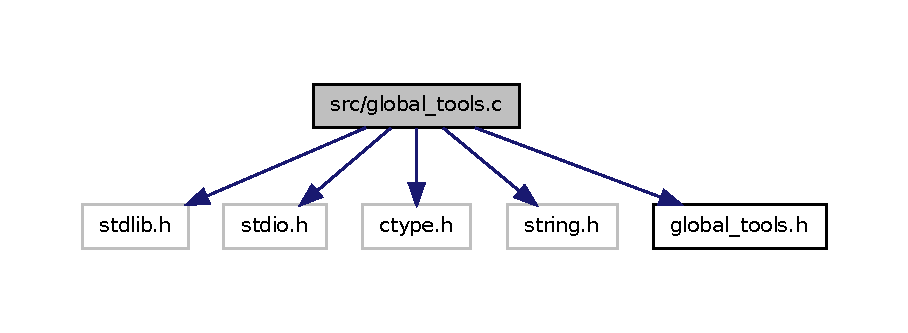
\includegraphics[width=400pt]{global__tools_8c__incl}
\end{center}
\end{figure}
\subsection*{Functions}
\begin{DoxyCompactItemize}
\item 
void \hyperlink{global__tools_8c_a2477f8984915fc015d7bd056300d2d99}{str\_\-toupper} (char string\mbox{[}$\,$\mbox{]})
\begin{DoxyCompactList}\small\item\em Converts a given string into upper case. \item\end{DoxyCompactList}\item 
void \hyperlink{global__tools_8c_a28b854fd4deffee93685888f1cb24e21}{my\_\-strcpy} (char destination\mbox{[}$\,$\mbox{]}, char source\mbox{[}$\,$\mbox{]}, int destination\_\-length)
\begin{DoxyCompactList}\small\item\em Safe form of string copy. \item\end{DoxyCompactList}\end{DoxyCompactItemize}


\subsection{Function Documentation}
\hypertarget{global__tools_8c_a28b854fd4deffee93685888f1cb24e21}{
\index{global\_\-tools.c@{global\_\-tools.c}!my\_\-strcpy@{my\_\-strcpy}}
\index{my\_\-strcpy@{my\_\-strcpy}!global_tools.c@{global\_\-tools.c}}
\subsubsection[{my\_\-strcpy}]{\setlength{\rightskip}{0pt plus 5cm}void my\_\-strcpy (
\begin{DoxyParamCaption}
\item[{char}]{ destination\mbox{[}$\,$\mbox{]}, }
\item[{char}]{ source\mbox{[}$\,$\mbox{]}, }
\item[{int}]{ destination\_\-length}
\end{DoxyParamCaption}
)}}
\label{global__tools_8c_a28b854fd4deffee93685888f1cb24e21}


Safe form of string copy. 

\hyperlink{global__tools_8c_a28b854fd4deffee93685888f1cb24e21}{my\_\-strcpy()} copies one string into another but does a size check before that.


\begin{DoxyParams}{Parameters}
\item[\mbox{\tt[out]} {\em destination}]string copied to \item[\mbox{\tt[in]} {\em source}]string copied from \item[\mbox{\tt[in]} {\em destination\_\-length}]length of destination buffer \end{DoxyParams}
\begin{DoxyReturn}{Returns}
nothing 
\end{DoxyReturn}
\begin{DoxySeeAlso}{See also}
Discussion of strncpy: \href{http://www.inspirel.com/articles/Strncpy_And_Safety.html}{\tt http://www.inspirel.com/articles/Strncpy\_\-And\_\-Safety.html} 

You cannot use sizeof here. See: \href{https://www.securecoding.cert.org/confluence/display/cplusplus/ARR01-CPP.+Do+not+apply+the+sizeof+operator+to+a+pointer+when+taking+the+size+of+an+array}{\tt CERT} 
\end{DoxySeeAlso}


Definition at line 42 of file global\_\-tools.c.




\begin{DoxyCode}
{
    if ( (int) strlen(source) <= destination_length ) {
        strcpy( destination, source );
    }
    else {
        fprintf( stderr, "Cannot copy destination string into source string\n");
        exit(1);
    }

    return;
}
\end{DoxyCode}


\hypertarget{global__tools_8c_a2477f8984915fc015d7bd056300d2d99}{
\index{global\_\-tools.c@{global\_\-tools.c}!str\_\-toupper@{str\_\-toupper}}
\index{str\_\-toupper@{str\_\-toupper}!global_tools.c@{global\_\-tools.c}}
\subsubsection[{str\_\-toupper}]{\setlength{\rightskip}{0pt plus 5cm}void str\_\-toupper (
\begin{DoxyParamCaption}
\item[{char}]{ string\mbox{[}$\,$\mbox{]}}
\end{DoxyParamCaption}
)}}
\label{global__tools_8c_a2477f8984915fc015d7bd056300d2d99}


Converts a given string into upper case. 

Converts a given string into upper case. The string is converted inplace. No copying is being done.


\begin{DoxyParams}{Parameters}
\item[\mbox{\tt[in]} {\em string}]a given string \end{DoxyParams}
\begin{DoxyReturn}{Returns}
nothing 
\end{DoxyReturn}
\begin{DoxySeeAlso}{See also}
\mbox{[}n/a\mbox{]} 
\end{DoxySeeAlso}


Definition at line 17 of file global\_\-tools.c.




\begin{DoxyCode}
{
    int i;
    int str_length = (int) strlen(string);

    for ( i = 0; i < str_length; i++ ) {
        string[i] = toupper( string[i] );
    }

    return;
}
\end{DoxyCode}



\hypertarget{global__tools_8h}{
\section{src/global\_\-tools.h File Reference}
\label{global__tools_8h}\index{src/global\_\-tools.h@{src/global\_\-tools.h}}
}
This graph shows which files directly or indirectly include this file:\nopagebreak
\begin{figure}[H]
\begin{center}
\leavevmode
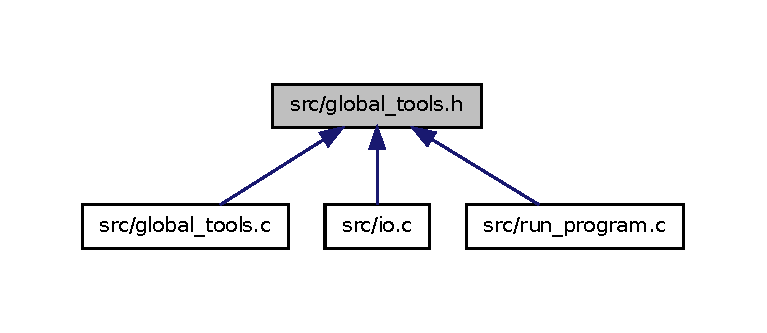
\includegraphics[width=368pt]{global__tools_8h__dep__incl}
\end{center}
\end{figure}
\subsection*{Functions}
\begin{DoxyCompactItemize}
\item 
void \hyperlink{global__tools_8h_a2477f8984915fc015d7bd056300d2d99}{str\_\-toupper} (char string\mbox{[}$\,$\mbox{]})
\begin{DoxyCompactList}\small\item\em Converts a given string into upper case. \item\end{DoxyCompactList}\item 
void \hyperlink{global__tools_8h_aee5d1003d9980671f97862e7c16a960d}{my\_\-strcpy} (char destination\mbox{[}$\,$\mbox{]}, char source\mbox{[}$\,$\mbox{]}, int desination\_\-length)
\begin{DoxyCompactList}\small\item\em Safe form of string copy. \item\end{DoxyCompactList}\end{DoxyCompactItemize}


\subsection{Function Documentation}
\hypertarget{global__tools_8h_aee5d1003d9980671f97862e7c16a960d}{
\index{global\_\-tools.h@{global\_\-tools.h}!my\_\-strcpy@{my\_\-strcpy}}
\index{my\_\-strcpy@{my\_\-strcpy}!global_tools.h@{global\_\-tools.h}}
\subsubsection[{my\_\-strcpy}]{\setlength{\rightskip}{0pt plus 5cm}void my\_\-strcpy (
\begin{DoxyParamCaption}
\item[{char}]{ destination\mbox{[}$\,$\mbox{]}, }
\item[{char}]{ source\mbox{[}$\,$\mbox{]}, }
\item[{int}]{ destination\_\-length}
\end{DoxyParamCaption}
)}}
\label{global__tools_8h_aee5d1003d9980671f97862e7c16a960d}


Safe form of string copy. 

\hyperlink{global__tools_8c_a28b854fd4deffee93685888f1cb24e21}{my\_\-strcpy()} copies one string into another but does a size check before that.


\begin{DoxyParams}{Parameters}
\item[\mbox{\tt[out]} {\em destination}]string copied to \item[\mbox{\tt[in]} {\em source}]string copied from \item[\mbox{\tt[in]} {\em destination\_\-length}]length of destination buffer \end{DoxyParams}
\begin{DoxyReturn}{Returns}
nothing 
\end{DoxyReturn}
\begin{DoxySeeAlso}{See also}
Discussion of strncpy: \href{http://www.inspirel.com/articles/Strncpy_And_Safety.html}{\tt http://www.inspirel.com/articles/Strncpy\_\-And\_\-Safety.html} 

You cannot use sizeof here. See: \href{https://www.securecoding.cert.org/confluence/display/cplusplus/ARR01-CPP.+Do+not+apply+the+sizeof+operator+to+a+pointer+when+taking+the+size+of+an+array}{\tt CERT} 
\end{DoxySeeAlso}


Definition at line 42 of file global\_\-tools.c.




\begin{DoxyCode}
{
    if ( (int) strlen(source) <= destination_length ) {
        strcpy( destination, source );
    }
    else {
        fprintf( stderr, "Cannot copy destination string into source string\n");
        exit(1);
    }

    return;
}
\end{DoxyCode}


\hypertarget{global__tools_8h_a2477f8984915fc015d7bd056300d2d99}{
\index{global\_\-tools.h@{global\_\-tools.h}!str\_\-toupper@{str\_\-toupper}}
\index{str\_\-toupper@{str\_\-toupper}!global_tools.h@{global\_\-tools.h}}
\subsubsection[{str\_\-toupper}]{\setlength{\rightskip}{0pt plus 5cm}void str\_\-toupper (
\begin{DoxyParamCaption}
\item[{char}]{ string\mbox{[}$\,$\mbox{]}}
\end{DoxyParamCaption}
)}}
\label{global__tools_8h_a2477f8984915fc015d7bd056300d2d99}


Converts a given string into upper case. 

Converts a given string into upper case. The string is converted inplace. No copying is being done.


\begin{DoxyParams}{Parameters}
\item[\mbox{\tt[in]} {\em string}]a given string \end{DoxyParams}
\begin{DoxyReturn}{Returns}
nothing 
\end{DoxyReturn}
\begin{DoxySeeAlso}{See also}
\mbox{[}n/a\mbox{]} 
\end{DoxySeeAlso}


Definition at line 17 of file global\_\-tools.c.




\begin{DoxyCode}
{
    int i;
    int str_length = (int) strlen(string);

    for ( i = 0; i < str_length; i++ ) {
        string[i] = toupper( string[i] );
    }

    return;
}
\end{DoxyCode}



\hypertarget{io_8c}{
\section{src/io.c File Reference}
\label{io_8c}\index{src/io.c@{src/io.c}}
}
{\ttfamily \#include $<$stdlib.h$>$}\par
{\ttfamily \#include $<$stdio.h$>$}\par
{\ttfamily \#include $<$string.h$>$}\par
{\ttfamily \#include $<$stdbool.h$>$}\par
{\ttfamily \#include $<$ctype.h$>$}\par
{\ttfamily \#include \char`\"{}global\_\-const.h\char`\"{}}\par
{\ttfamily \#include \char`\"{}io.h\char`\"{}}\par
{\ttfamily \#include \char`\"{}global\_\-tools.h\char`\"{}}\par
Include dependency graph for io.c:\nopagebreak
\begin{figure}[H]
\begin{center}
\leavevmode
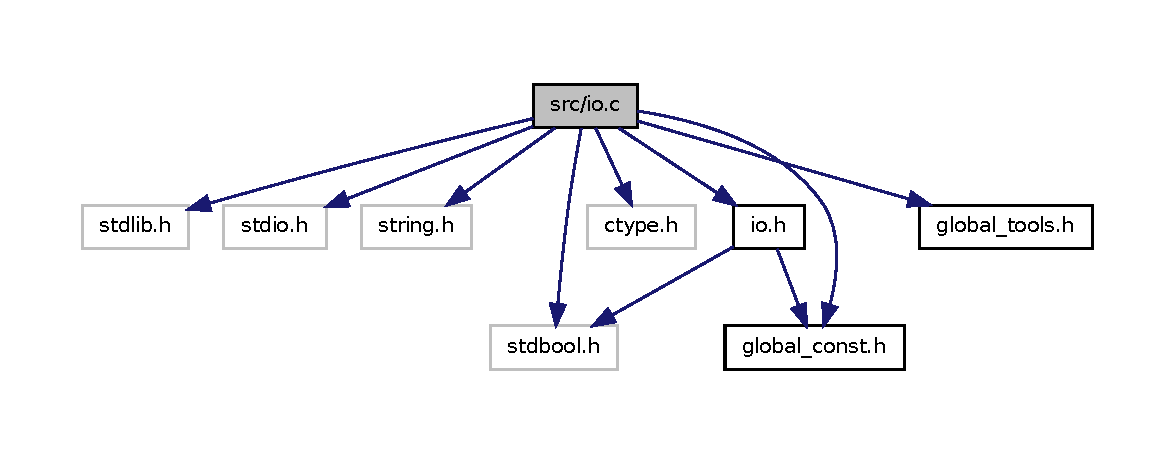
\includegraphics[width=400pt]{io_8c__incl}
\end{center}
\end{figure}
\subsection*{Functions}
\begin{DoxyCompactItemize}
\item 
void \hyperlink{io_8c_af6dafebf6767ddb1f453059f63968cfa}{read\_\-gtp\_\-input} (struct \hyperlink{structcommand}{command} $\ast$command\_\-data)
\begin{DoxyCompactList}\small\item\em Read GTP command from STDIN. \item\end{DoxyCompactList}\item 
void \hyperlink{io_8c_a2b37ea825b377573cc5ba1926636fac7}{set\_\-output\_\-error} (void)
\item 
bool \hyperlink{io_8c_a2a55445d2f8582b642b0812b3350b7b4}{get\_\-output\_\-error} (void)
\item 
void \hyperlink{io_8c_add90506be30c4ba9e5be8a6c3c6490a3}{add\_\-output} (const char to\_\-output\mbox{[}$\,$\mbox{]})
\item 
void \hyperlink{io_8c_a84addba8fd5fd0fad9e2f8727ef48127}{print\_\-output} (int command\_\-id)
\item 
void \hyperlink{io_8c_a0268c75a0ce2925365247fb5840392d2}{trim} (char $\ast$input)
\item 
void \hyperlink{io_8c_a67efb5aef9656c26f6bc14c91ca1bbba}{drop\_\-comment} (char $\ast$input)
\item 
bool \hyperlink{io_8c_a65a3f2710b61f5e5a38f6439be41b29a}{is\_\-input\_\-empty} (void)
\item 
void \hyperlink{io_8c_a94c0ca601c65a0c12e8388856af0b9d3}{parse\_\-gtp\_\-input} (char $\ast$\hyperlink{io_8c_a6b224d51bbc57f2a09a055e2345cda8e}{command\_\-input\_\-buffer}, char tokens\mbox{[}$\,$\mbox{]}\mbox{[}MAX\_\-TOKEN\_\-LENGTH\mbox{]})
\item 
void \hyperlink{io_8c_a264f14a49c3575cdd898f81e03243a3c}{init\_\-tokens} (char tokens\mbox{[}$\,$\mbox{]}\mbox{[}MAX\_\-TOKEN\_\-LENGTH\mbox{]})
\item 
void \hyperlink{io_8c_a953fa7252e26e5c019ccef5e98682678}{identify\_\-tokens} (char tokens\mbox{[}$\,$\mbox{]}\mbox{[}MAX\_\-TOKEN\_\-LENGTH\mbox{]}, struct \hyperlink{structcommand}{command} $\ast$command\_\-data)
\end{DoxyCompactItemize}
\subsection*{Variables}
\begin{DoxyCompactItemize}
\item 
char \hyperlink{io_8c_a6b224d51bbc57f2a09a055e2345cda8e}{command\_\-input\_\-buffer} \mbox{[}SIZE\_\-INPUT\_\-BUFFER\mbox{]}
\item 
bool \hyperlink{io_8c_a11a728181e103926141fc71fb7eaaec6}{input\_\-empty} = false
\item 
bool \hyperlink{io_8c_a9f66eed02223981a4d085f8ce0a2bdd1}{output\_\-error} = false
\item 
char \hyperlink{io_8c_a8eebc622d86f8c1aea9657171cb93b13}{output} \mbox{[}MAX\_\-OUTPUT\_\-LENGTH\mbox{]}
\end{DoxyCompactItemize}


\subsection{Function Documentation}
\hypertarget{io_8c_add90506be30c4ba9e5be8a6c3c6490a3}{
\index{io.c@{io.c}!add\_\-output@{add\_\-output}}
\index{add\_\-output@{add\_\-output}!io.c@{io.c}}
\subsubsection[{add\_\-output}]{\setlength{\rightskip}{0pt plus 5cm}void add\_\-output (
\begin{DoxyParamCaption}
\item[{const char}]{ to\_\-output\mbox{[}$\,$\mbox{]}}
\end{DoxyParamCaption}
)}}
\label{io_8c_add90506be30c4ba9e5be8a6c3c6490a3}


Definition at line 115 of file io.c.




\begin{DoxyCode}
                                          {

    int new_output_length
        = (int)( strlen(output) + strlen(to_output) + 1 );
    if ( new_output_length > MAX_OUTPUT_LENGTH ) {
        fprintf( stderr, "MAX_OUTPUT_LENGTH exceeded\n" );
        exit(EXIT_FAILURE);
    }

    strcat( output, to_output );
    strcat( output, "\n" );

    return;
}
\end{DoxyCode}


\hypertarget{io_8c_a67efb5aef9656c26f6bc14c91ca1bbba}{
\index{io.c@{io.c}!drop\_\-comment@{drop\_\-comment}}
\index{drop\_\-comment@{drop\_\-comment}!io.c@{io.c}}
\subsubsection[{drop\_\-comment}]{\setlength{\rightskip}{0pt plus 5cm}void drop\_\-comment (
\begin{DoxyParamCaption}
\item[{char $\ast$}]{ input}
\end{DoxyParamCaption}
)}}
\label{io_8c_a67efb5aef9656c26f6bc14c91ca1bbba}


Definition at line 233 of file io.c.




\begin{DoxyCode}
                                  {
    int i = 0;
    char current_char = '\0';

    for ( i = 0; i < SIZE_INPUT_BUFFER; i++ ) {
        current_char = input[i];
        if ( current_char == '#' ) {
            input[i] = '\0';
            break;
        }
        if ( current_char == '\0' ) {
            break;
        }
    }

    return;
}
\end{DoxyCode}


\hypertarget{io_8c_a2a55445d2f8582b642b0812b3350b7b4}{
\index{io.c@{io.c}!get\_\-output\_\-error@{get\_\-output\_\-error}}
\index{get\_\-output\_\-error@{get\_\-output\_\-error}!io.c@{io.c}}
\subsubsection[{get\_\-output\_\-error}]{\setlength{\rightskip}{0pt plus 5cm}bool get\_\-output\_\-error (
\begin{DoxyParamCaption}
\item[{void}]{}
\end{DoxyParamCaption}
)}}
\label{io_8c_a2a55445d2f8582b642b0812b3350b7b4}


Definition at line 100 of file io.c.




\begin{DoxyCode}
                            {

    return output_error;
}
\end{DoxyCode}


\hypertarget{io_8c_a953fa7252e26e5c019ccef5e98682678}{
\index{io.c@{io.c}!identify\_\-tokens@{identify\_\-tokens}}
\index{identify\_\-tokens@{identify\_\-tokens}!io.c@{io.c}}
\subsubsection[{identify\_\-tokens}]{\setlength{\rightskip}{0pt plus 5cm}void identify\_\-tokens (
\begin{DoxyParamCaption}
\item[{char}]{ tokens\mbox{[}$\,$\mbox{]}\mbox{[}MAX\_\-TOKEN\_\-LENGTH\mbox{]}, }
\item[{struct {\bf command} $\ast$}]{ command\_\-data}
\end{DoxyParamCaption}
)}}
\label{io_8c_a953fa7252e26e5c019ccef5e98682678}


Definition at line 350 of file io.c.




\begin{DoxyCode}
                                                                                 
           {
    int id;
    int arg_start;  // Index of first argument
    int i, j;

    // Check if first token is regular id,
    // if not it must be the command name.
    id = atoi( tokens[0] );
    if ( id > 0 ) {
        command_data->id = id;
        my_strcpy( command_data->name, tokens[1], MAX_TOKEN_LENGTH );
        arg_start = 2;
    }
    else if ( id < 0 ) {
        command_data->id = -1;
        my_strcpy( command_data->name, tokens[1], MAX_TOKEN_LENGTH );
        arg_start = 2;
    }
    else {
        command_data->id = -1;
        my_strcpy( command_data->name, tokens[0], MAX_TOKEN_LENGTH );
        arg_start = 1;
    }

    // Check for special case id 0:
    if ( strcmp( tokens[0], "0" ) == 0 ) {
        command_data->id = 0;
        my_strcpy( command_data->name, tokens[1], MAX_TOKEN_LENGTH );
        arg_start = 2;
    }

    // Copy arguments into command struct:
    j = 0;
    for ( i = arg_start; i < MAX_TOKEN_COUNT; i++ ) {
        if ( tokens[i][0] == '\0' ) {
            break;
        }
        my_strcpy( command_data->gtp_argv[j], tokens[i], MAX_TOKEN_LENGTH );
        j++;
    }
    command_data->gtp_argc = j;

    // Add terminating argument:
    my_strcpy( command_data->gtp_argv[j], "\0", MAX_TOKEN_LENGTH );

    // DEBUG
    /*
    printf( "ID: %d\n", command_data->id );
    printf( "NAME: %s\n", command_data->name );
    printf( "ARGC: %d\n", command_data->argc );
    for ( i = 0; i < j; i++ ) {
        printf( "ARG %d: %s\n", i, command_data->argv[i] );
    }
    */

    return;
}
\end{DoxyCode}


\hypertarget{io_8c_a264f14a49c3575cdd898f81e03243a3c}{
\index{io.c@{io.c}!init\_\-tokens@{init\_\-tokens}}
\index{init\_\-tokens@{init\_\-tokens}!io.c@{io.c}}
\subsubsection[{init\_\-tokens}]{\setlength{\rightskip}{0pt plus 5cm}void init\_\-tokens (
\begin{DoxyParamCaption}
\item[{char}]{ tokens\mbox{[}$\,$\mbox{]}\mbox{[}MAX\_\-TOKEN\_\-LENGTH\mbox{]}}
\end{DoxyParamCaption}
)}}
\label{io_8c_a264f14a49c3575cdd898f81e03243a3c}


Definition at line 329 of file io.c.




\begin{DoxyCode}
                                                    {
    int i;

    for ( i = 0; i < MAX_TOKEN_COUNT; i++ ) {
        tokens[i][0] = '\0';
    }

    return;
}
\end{DoxyCode}


\hypertarget{io_8c_a65a3f2710b61f5e5a38f6439be41b29a}{
\index{io.c@{io.c}!is\_\-input\_\-empty@{is\_\-input\_\-empty}}
\index{is\_\-input\_\-empty@{is\_\-input\_\-empty}!io.c@{io.c}}
\subsubsection[{is\_\-input\_\-empty}]{\setlength{\rightskip}{0pt plus 5cm}bool is\_\-input\_\-empty (
\begin{DoxyParamCaption}
\item[{void}]{}
\end{DoxyParamCaption}
)}}
\label{io_8c_a65a3f2710b61f5e5a38f6439be41b29a}


Definition at line 260 of file io.c.




\begin{DoxyCode}
                          {

    return input_empty;
}
\end{DoxyCode}


\hypertarget{io_8c_a94c0ca601c65a0c12e8388856af0b9d3}{
\index{io.c@{io.c}!parse\_\-gtp\_\-input@{parse\_\-gtp\_\-input}}
\index{parse\_\-gtp\_\-input@{parse\_\-gtp\_\-input}!io.c@{io.c}}
\subsubsection[{parse\_\-gtp\_\-input}]{\setlength{\rightskip}{0pt plus 5cm}void parse\_\-gtp\_\-input (
\begin{DoxyParamCaption}
\item[{char $\ast$}]{ command\_\-input\_\-buffer, }
\item[{char}]{ tokens\mbox{[}$\,$\mbox{]}\mbox{[}MAX\_\-TOKEN\_\-LENGTH\mbox{]}}
\end{DoxyParamCaption}
)}}
\label{io_8c_a94c0ca601c65a0c12e8388856af0b9d3}


Definition at line 275 of file io.c.




\begin{DoxyCode}
                                                                                 
          {
    char current_char = '\0';
    int i = 0;  // Index of input buffer
    int j = 0;  // Counts number of tokens
    int k = 0;  // Index of each token

    // Get tokens from input:
    for ( i = 0; i < SIZE_INPUT_BUFFER; i++ ) {
        current_char = command_input_buffer[i];
        if ( ! isspace(current_char) && current_char != '\0' ) {
            if ( k < MAX_TOKEN_LENGTH ) {
                tokens[j][k] = current_char;
                k++;
            }
            else {
                set_output_error();
                add_output( "MAX_TOKEN_LENGTH exceeded" );
                init_tokens(tokens);
                return;
            }
        }
        else {
            tokens[j][k] = '\0';
            j++;
            k = 0;

            if ( j >= MAX_TOKEN_COUNT ) {
                set_output_error();
                add_output( "MAX_TOKEN_COUNT exceeded" );
                init_tokens(tokens);
                return;
            }

            // Set terminating argument:
            tokens[j][0] = '\0';
        }

        if ( current_char == '\0' ) {
            break;
        }
    }

    return;
}
\end{DoxyCode}


\hypertarget{io_8c_a84addba8fd5fd0fad9e2f8727ef48127}{
\index{io.c@{io.c}!print\_\-output@{print\_\-output}}
\index{print\_\-output@{print\_\-output}!io.c@{io.c}}
\subsubsection[{print\_\-output}]{\setlength{\rightskip}{0pt plus 5cm}void print\_\-output (
\begin{DoxyParamCaption}
\item[{int}]{ command\_\-id}
\end{DoxyParamCaption}
)}}
\label{io_8c_a84addba8fd5fd0fad9e2f8727ef48127}


Definition at line 140 of file io.c.




\begin{DoxyCode}
                                    {

    /*
    if ( input_empty == true ) {
        input_empty = false;
        return;
    }
    */

    if ( output_error == false ) {
        printf("=");
    }
    else {
        printf("?");
    }

    if ( command_id >= 0 ) {
        printf( "%d", command_id );
    }

    printf(" ");
    
    // If output is empty we fill it with an empty string to
    // get that additional newline:
    if ( strlen(output) == 0 ) {
        add_output("");
    }

    printf( "%s\n", output );

    my_strcpy( output, "", MAX_OUTPUT_LENGTH );
    //output_error = false;

    return;
}
\end{DoxyCode}


\hypertarget{io_8c_af6dafebf6767ddb1f453059f63968cfa}{
\index{io.c@{io.c}!read\_\-gtp\_\-input@{read\_\-gtp\_\-input}}
\index{read\_\-gtp\_\-input@{read\_\-gtp\_\-input}!io.c@{io.c}}
\subsubsection[{read\_\-gtp\_\-input}]{\setlength{\rightskip}{0pt plus 5cm}void read\_\-gtp\_\-input (
\begin{DoxyParamCaption}
\item[{struct {\bf command} $\ast$}]{ command\_\-data}
\end{DoxyParamCaption}
)}}
\label{io_8c_af6dafebf6767ddb1f453059f63968cfa}


Read GTP command from STDIN. 

Reads a GTP command from STDIN. Input which is larger than SIZE\_\-INPUT\_\-BUFFER is simply ignored. The behaviour {\itshape should\/} be the same as with \char`\"{}gnugo -\/-\/mode gtp\char`\"{}.


\begin{DoxyParams}{Parameters}
\item[\mbox{\tt[in]} {\em $\ast$command\_\-data}]Pointer to struct command \end{DoxyParams}
\begin{DoxyReturn}{Returns}
nothing 
\end{DoxyReturn}
\begin{DoxySeeAlso}{See also}
\href{http://www.lysator.liu.se/~gunnar/gtp/}{\tt GTP version 2.0} 
\end{DoxySeeAlso}


Definition at line 40 of file io.c.




\begin{DoxyCode}
{
    int c = '\n';
    int i = 0;
    char tokens[MAX_TOKEN_COUNT][MAX_TOKEN_LENGTH];

    init_tokens(tokens);

    input_empty  = false;
    output_error = false;

    do {
        c = getchar();
        command_input_buffer[i] = (char) c;
        i++;
    } while ( c != '\n' && i < SIZE_INPUT_BUFFER );

    // Overwrite last char with newline
    command_input_buffer[i-1] = '\0';

    drop_comment(command_input_buffer);
    trim(command_input_buffer);

    if ( strlen(command_input_buffer) == 0 ) {
        input_empty = true;
        return;
    }

    parse_gtp_input( command_input_buffer, tokens );
    identify_tokens( tokens, command_data );

    return;
}
\end{DoxyCode}


\hypertarget{io_8c_a2b37ea825b377573cc5ba1926636fac7}{
\index{io.c@{io.c}!set\_\-output\_\-error@{set\_\-output\_\-error}}
\index{set\_\-output\_\-error@{set\_\-output\_\-error}!io.c@{io.c}}
\subsubsection[{set\_\-output\_\-error}]{\setlength{\rightskip}{0pt plus 5cm}void set\_\-output\_\-error (
\begin{DoxyParamCaption}
\item[{void}]{}
\end{DoxyParamCaption}
)}}
\label{io_8c_a2b37ea825b377573cc5ba1926636fac7}


Definition at line 84 of file io.c.




\begin{DoxyCode}
                            {

    output_error = true;

    return;
}
\end{DoxyCode}


\hypertarget{io_8c_a0268c75a0ce2925365247fb5840392d2}{
\index{io.c@{io.c}!trim@{trim}}
\index{trim@{trim}!io.c@{io.c}}
\subsubsection[{trim}]{\setlength{\rightskip}{0pt plus 5cm}void trim (
\begin{DoxyParamCaption}
\item[{char $\ast$}]{ input}
\end{DoxyParamCaption}
)}}
\label{io_8c_a0268c75a0ce2925365247fb5840392d2}


Definition at line 187 of file io.c.




\begin{DoxyCode}
                          {
    char temp_input[SIZE_INPUT_BUFFER];
    char current_char = '\0';
    char last_char    = '\0';
    int i = 0;
    int j = 0;

    for ( i = 0; i < SIZE_INPUT_BUFFER; i++ ) {
        current_char = input[i];

        /* Skip leading whitespace */
        if ( isspace(current_char) && j == 0 ) {
            continue;
        }
        
        /* Write only one whitespace */
        if ( isspace(last_char) && !isspace(current_char) && current_char != '\0'
       ) {
            temp_input[j] = ' ';
            j++;
        }

        /* Write non-whitespace characters */
        if ( ! isspace(current_char) ) {
            temp_input[j] = current_char;
            j++;
        }

        last_char = current_char;
    }

    temp_input[j] = '\0';

    strncpy( input, temp_input, SIZE_INPUT_BUFFER );

    return;
}
\end{DoxyCode}




\subsection{Variable Documentation}
\hypertarget{io_8c_a6b224d51bbc57f2a09a055e2345cda8e}{
\index{io.c@{io.c}!command\_\-input\_\-buffer@{command\_\-input\_\-buffer}}
\index{command\_\-input\_\-buffer@{command\_\-input\_\-buffer}!io.c@{io.c}}
\subsubsection[{command\_\-input\_\-buffer}]{\setlength{\rightskip}{0pt plus 5cm}char {\bf command\_\-input\_\-buffer}\mbox{[}SIZE\_\-INPUT\_\-BUFFER\mbox{]}}}
\label{io_8c_a6b224d51bbc57f2a09a055e2345cda8e}


Definition at line 10 of file io.c.

\hypertarget{io_8c_a11a728181e103926141fc71fb7eaaec6}{
\index{io.c@{io.c}!input\_\-empty@{input\_\-empty}}
\index{input\_\-empty@{input\_\-empty}!io.c@{io.c}}
\subsubsection[{input\_\-empty}]{\setlength{\rightskip}{0pt plus 5cm}bool {\bf input\_\-empty} = false}}
\label{io_8c_a11a728181e103926141fc71fb7eaaec6}


Definition at line 12 of file io.c.

\hypertarget{io_8c_a8eebc622d86f8c1aea9657171cb93b13}{
\index{io.c@{io.c}!output@{output}}
\index{output@{output}!io.c@{io.c}}
\subsubsection[{output}]{\setlength{\rightskip}{0pt plus 5cm}char {\bf output}\mbox{[}MAX\_\-OUTPUT\_\-LENGTH\mbox{]}}}
\label{io_8c_a8eebc622d86f8c1aea9657171cb93b13}


Definition at line 14 of file io.c.

\hypertarget{io_8c_a9f66eed02223981a4d085f8ce0a2bdd1}{
\index{io.c@{io.c}!output\_\-error@{output\_\-error}}
\index{output\_\-error@{output\_\-error}!io.c@{io.c}}
\subsubsection[{output\_\-error}]{\setlength{\rightskip}{0pt plus 5cm}bool {\bf output\_\-error} = false}}
\label{io_8c_a9f66eed02223981a4d085f8ce0a2bdd1}


Definition at line 13 of file io.c.


\hypertarget{io_8h}{
\section{src/io.h File Reference}
\label{io_8h}\index{src/io.h@{src/io.h}}
}
{\ttfamily \#include $<$stdbool.h$>$}\par
{\ttfamily \#include \char`\"{}global\_\-const.h\char`\"{}}\par
Include dependency graph for io.h:\nopagebreak
\begin{figure}[H]
\begin{center}
\leavevmode
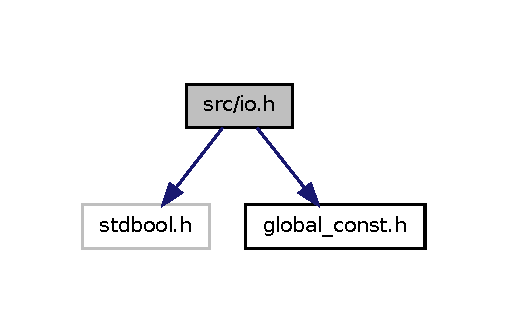
\includegraphics[width=244pt]{io_8h__incl}
\end{center}
\end{figure}
This graph shows which files directly or indirectly include this file:\nopagebreak
\begin{figure}[H]
\begin{center}
\leavevmode
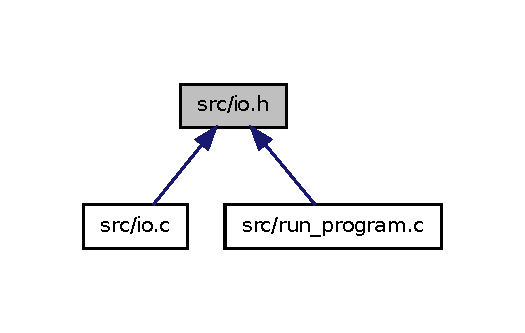
\includegraphics[width=252pt]{io_8h__dep__incl}
\end{center}
\end{figure}
\subsection*{Data Structures}
\begin{DoxyCompactItemize}
\item 
struct \hyperlink{structcommand}{command}
\end{DoxyCompactItemize}
\subsection*{Defines}
\begin{DoxyCompactItemize}
\item 
\#define \hyperlink{io_8h_a6bf23a007255bce0fe1fd922130f6cd6}{SIZE\_\-INPUT\_\-BUFFER}~256
\end{DoxyCompactItemize}
\subsection*{Functions}
\begin{DoxyCompactItemize}
\item 
void \hyperlink{io_8h_af6dafebf6767ddb1f453059f63968cfa}{read\_\-gtp\_\-input} (struct \hyperlink{structcommand}{command} $\ast$command\_\-data)
\begin{DoxyCompactList}\small\item\em Read GTP command from STDIN. \item\end{DoxyCompactList}\item 
void \hyperlink{io_8h_add90506be30c4ba9e5be8a6c3c6490a3}{add\_\-output} (const char to\_\-output\mbox{[}$\,$\mbox{]})
\item 
void \hyperlink{io_8h_a2b37ea825b377573cc5ba1926636fac7}{set\_\-output\_\-error} (void)
\item 
bool \hyperlink{io_8h_a2a55445d2f8582b642b0812b3350b7b4}{get\_\-output\_\-error} (void)
\item 
void \hyperlink{io_8h_a84addba8fd5fd0fad9e2f8727ef48127}{print\_\-output} (int command\_\-id)
\item 
void \hyperlink{io_8h_a0268c75a0ce2925365247fb5840392d2}{trim} (char $\ast$input)
\item 
void \hyperlink{io_8h_a67efb5aef9656c26f6bc14c91ca1bbba}{drop\_\-comment} (char $\ast$input)
\item 
void \hyperlink{io_8h_afb4d7e594c7910a1e528dd826cdde2bf}{parse\_\-gtp\_\-input} (char $\ast$\hyperlink{io_8c_a6b224d51bbc57f2a09a055e2345cda8e}{command\_\-input\_\-buffer}, char \hyperlink{structcommand}{command}\mbox{[}$\,$\mbox{]}\mbox{[}MAX\_\-TOKEN\_\-LENGTH\mbox{]})
\item 
void \hyperlink{io_8h_a264f14a49c3575cdd898f81e03243a3c}{init\_\-tokens} (char tokens\mbox{[}$\,$\mbox{]}\mbox{[}MAX\_\-TOKEN\_\-LENGTH\mbox{]})
\item 
void \hyperlink{io_8h_a953fa7252e26e5c019ccef5e98682678}{identify\_\-tokens} (char tokens\mbox{[}$\,$\mbox{]}\mbox{[}MAX\_\-TOKEN\_\-LENGTH\mbox{]}, struct \hyperlink{structcommand}{command} $\ast$command\_\-data)
\item 
bool \hyperlink{io_8h_a65a3f2710b61f5e5a38f6439be41b29a}{is\_\-input\_\-empty} (void)
\end{DoxyCompactItemize}


\subsection{Define Documentation}
\hypertarget{io_8h_a6bf23a007255bce0fe1fd922130f6cd6}{
\index{io.h@{io.h}!SIZE\_\-INPUT\_\-BUFFER@{SIZE\_\-INPUT\_\-BUFFER}}
\index{SIZE\_\-INPUT\_\-BUFFER@{SIZE\_\-INPUT\_\-BUFFER}!io.h@{io.h}}
\subsubsection[{SIZE\_\-INPUT\_\-BUFFER}]{\setlength{\rightskip}{0pt plus 5cm}\#define SIZE\_\-INPUT\_\-BUFFER~256}}
\label{io_8h_a6bf23a007255bce0fe1fd922130f6cd6}


Definition at line 7 of file io.h.



\subsection{Function Documentation}
\hypertarget{io_8h_add90506be30c4ba9e5be8a6c3c6490a3}{
\index{io.h@{io.h}!add\_\-output@{add\_\-output}}
\index{add\_\-output@{add\_\-output}!io.h@{io.h}}
\subsubsection[{add\_\-output}]{\setlength{\rightskip}{0pt plus 5cm}void add\_\-output (
\begin{DoxyParamCaption}
\item[{const char}]{ to\_\-output\mbox{[}$\,$\mbox{]}}
\end{DoxyParamCaption}
)}}
\label{io_8h_add90506be30c4ba9e5be8a6c3c6490a3}


Definition at line 115 of file io.c.




\begin{DoxyCode}
                                          {

    int new_output_length
        = (int)( strlen(output) + strlen(to_output) + 1 );
    if ( new_output_length > MAX_OUTPUT_LENGTH ) {
        fprintf( stderr, "MAX_OUTPUT_LENGTH exceeded\n" );
        exit(EXIT_FAILURE);
    }

    strcat( output, to_output );
    strcat( output, "\n" );

    return;
}
\end{DoxyCode}


\hypertarget{io_8h_a67efb5aef9656c26f6bc14c91ca1bbba}{
\index{io.h@{io.h}!drop\_\-comment@{drop\_\-comment}}
\index{drop\_\-comment@{drop\_\-comment}!io.h@{io.h}}
\subsubsection[{drop\_\-comment}]{\setlength{\rightskip}{0pt plus 5cm}void drop\_\-comment (
\begin{DoxyParamCaption}
\item[{char $\ast$}]{ input}
\end{DoxyParamCaption}
)}}
\label{io_8h_a67efb5aef9656c26f6bc14c91ca1bbba}


Definition at line 233 of file io.c.




\begin{DoxyCode}
                                  {
    int i = 0;
    char current_char = '\0';

    for ( i = 0; i < SIZE_INPUT_BUFFER; i++ ) {
        current_char = input[i];
        if ( current_char == '#' ) {
            input[i] = '\0';
            break;
        }
        if ( current_char == '\0' ) {
            break;
        }
    }

    return;
}
\end{DoxyCode}


\hypertarget{io_8h_a2a55445d2f8582b642b0812b3350b7b4}{
\index{io.h@{io.h}!get\_\-output\_\-error@{get\_\-output\_\-error}}
\index{get\_\-output\_\-error@{get\_\-output\_\-error}!io.h@{io.h}}
\subsubsection[{get\_\-output\_\-error}]{\setlength{\rightskip}{0pt plus 5cm}bool get\_\-output\_\-error (
\begin{DoxyParamCaption}
\item[{void}]{}
\end{DoxyParamCaption}
)}}
\label{io_8h_a2a55445d2f8582b642b0812b3350b7b4}


Definition at line 100 of file io.c.




\begin{DoxyCode}
                            {

    return output_error;
}
\end{DoxyCode}


\hypertarget{io_8h_a953fa7252e26e5c019ccef5e98682678}{
\index{io.h@{io.h}!identify\_\-tokens@{identify\_\-tokens}}
\index{identify\_\-tokens@{identify\_\-tokens}!io.h@{io.h}}
\subsubsection[{identify\_\-tokens}]{\setlength{\rightskip}{0pt plus 5cm}void identify\_\-tokens (
\begin{DoxyParamCaption}
\item[{char}]{ tokens\mbox{[}$\,$\mbox{]}\mbox{[}MAX\_\-TOKEN\_\-LENGTH\mbox{]}, }
\item[{struct {\bf command} $\ast$}]{ command\_\-data}
\end{DoxyParamCaption}
)}}
\label{io_8h_a953fa7252e26e5c019ccef5e98682678}


Definition at line 350 of file io.c.




\begin{DoxyCode}
                                                                                 
           {
    int id;
    int arg_start;  // Index of first argument
    int i, j;

    // Check if first token is regular id,
    // if not it must be the command name.
    id = atoi( tokens[0] );
    if ( id > 0 ) {
        command_data->id = id;
        my_strcpy( command_data->name, tokens[1], MAX_TOKEN_LENGTH );
        arg_start = 2;
    }
    else if ( id < 0 ) {
        command_data->id = -1;
        my_strcpy( command_data->name, tokens[1], MAX_TOKEN_LENGTH );
        arg_start = 2;
    }
    else {
        command_data->id = -1;
        my_strcpy( command_data->name, tokens[0], MAX_TOKEN_LENGTH );
        arg_start = 1;
    }

    // Check for special case id 0:
    if ( strcmp( tokens[0], "0" ) == 0 ) {
        command_data->id = 0;
        my_strcpy( command_data->name, tokens[1], MAX_TOKEN_LENGTH );
        arg_start = 2;
    }

    // Copy arguments into command struct:
    j = 0;
    for ( i = arg_start; i < MAX_TOKEN_COUNT; i++ ) {
        if ( tokens[i][0] == '\0' ) {
            break;
        }
        my_strcpy( command_data->gtp_argv[j], tokens[i], MAX_TOKEN_LENGTH );
        j++;
    }
    command_data->gtp_argc = j;

    // Add terminating argument:
    my_strcpy( command_data->gtp_argv[j], "\0", MAX_TOKEN_LENGTH );

    // DEBUG
    /*
    printf( "ID: %d\n", command_data->id );
    printf( "NAME: %s\n", command_data->name );
    printf( "ARGC: %d\n", command_data->argc );
    for ( i = 0; i < j; i++ ) {
        printf( "ARG %d: %s\n", i, command_data->argv[i] );
    }
    */

    return;
}
\end{DoxyCode}


\hypertarget{io_8h_a264f14a49c3575cdd898f81e03243a3c}{
\index{io.h@{io.h}!init\_\-tokens@{init\_\-tokens}}
\index{init\_\-tokens@{init\_\-tokens}!io.h@{io.h}}
\subsubsection[{init\_\-tokens}]{\setlength{\rightskip}{0pt plus 5cm}void init\_\-tokens (
\begin{DoxyParamCaption}
\item[{char}]{ tokens\mbox{[}$\,$\mbox{]}\mbox{[}MAX\_\-TOKEN\_\-LENGTH\mbox{]}}
\end{DoxyParamCaption}
)}}
\label{io_8h_a264f14a49c3575cdd898f81e03243a3c}


Definition at line 329 of file io.c.




\begin{DoxyCode}
                                                    {
    int i;

    for ( i = 0; i < MAX_TOKEN_COUNT; i++ ) {
        tokens[i][0] = '\0';
    }

    return;
}
\end{DoxyCode}


\hypertarget{io_8h_a65a3f2710b61f5e5a38f6439be41b29a}{
\index{io.h@{io.h}!is\_\-input\_\-empty@{is\_\-input\_\-empty}}
\index{is\_\-input\_\-empty@{is\_\-input\_\-empty}!io.h@{io.h}}
\subsubsection[{is\_\-input\_\-empty}]{\setlength{\rightskip}{0pt plus 5cm}bool is\_\-input\_\-empty (
\begin{DoxyParamCaption}
\item[{void}]{}
\end{DoxyParamCaption}
)}}
\label{io_8h_a65a3f2710b61f5e5a38f6439be41b29a}


Definition at line 260 of file io.c.




\begin{DoxyCode}
                          {

    return input_empty;
}
\end{DoxyCode}


\hypertarget{io_8h_afb4d7e594c7910a1e528dd826cdde2bf}{
\index{io.h@{io.h}!parse\_\-gtp\_\-input@{parse\_\-gtp\_\-input}}
\index{parse\_\-gtp\_\-input@{parse\_\-gtp\_\-input}!io.h@{io.h}}
\subsubsection[{parse\_\-gtp\_\-input}]{\setlength{\rightskip}{0pt plus 5cm}void parse\_\-gtp\_\-input (
\begin{DoxyParamCaption}
\item[{char $\ast$}]{ command\_\-input\_\-buffer, }
\item[{char}]{ command\mbox{[}$\,$\mbox{]}\mbox{[}MAX\_\-TOKEN\_\-LENGTH\mbox{]}}
\end{DoxyParamCaption}
)}}
\label{io_8h_afb4d7e594c7910a1e528dd826cdde2bf}


Definition at line 275 of file io.c.




\begin{DoxyCode}
                                                                                 
          {
    char current_char = '\0';
    int i = 0;  // Index of input buffer
    int j = 0;  // Counts number of tokens
    int k = 0;  // Index of each token

    // Get tokens from input:
    for ( i = 0; i < SIZE_INPUT_BUFFER; i++ ) {
        current_char = command_input_buffer[i];
        if ( ! isspace(current_char) && current_char != '\0' ) {
            if ( k < MAX_TOKEN_LENGTH ) {
                tokens[j][k] = current_char;
                k++;
            }
            else {
                set_output_error();
                add_output( "MAX_TOKEN_LENGTH exceeded" );
                init_tokens(tokens);
                return;
            }
        }
        else {
            tokens[j][k] = '\0';
            j++;
            k = 0;

            if ( j >= MAX_TOKEN_COUNT ) {
                set_output_error();
                add_output( "MAX_TOKEN_COUNT exceeded" );
                init_tokens(tokens);
                return;
            }

            // Set terminating argument:
            tokens[j][0] = '\0';
        }

        if ( current_char == '\0' ) {
            break;
        }
    }

    return;
}
\end{DoxyCode}


\hypertarget{io_8h_a84addba8fd5fd0fad9e2f8727ef48127}{
\index{io.h@{io.h}!print\_\-output@{print\_\-output}}
\index{print\_\-output@{print\_\-output}!io.h@{io.h}}
\subsubsection[{print\_\-output}]{\setlength{\rightskip}{0pt plus 5cm}void print\_\-output (
\begin{DoxyParamCaption}
\item[{int}]{ command\_\-id}
\end{DoxyParamCaption}
)}}
\label{io_8h_a84addba8fd5fd0fad9e2f8727ef48127}


Definition at line 140 of file io.c.




\begin{DoxyCode}
                                    {

    /*
    if ( input_empty == true ) {
        input_empty = false;
        return;
    }
    */

    if ( output_error == false ) {
        printf("=");
    }
    else {
        printf("?");
    }

    if ( command_id >= 0 ) {
        printf( "%d", command_id );
    }

    printf(" ");
    
    // If output is empty we fill it with an empty string to
    // get that additional newline:
    if ( strlen(output) == 0 ) {
        add_output("");
    }

    printf( "%s\n", output );

    my_strcpy( output, "", MAX_OUTPUT_LENGTH );
    //output_error = false;

    return;
}
\end{DoxyCode}


\hypertarget{io_8h_af6dafebf6767ddb1f453059f63968cfa}{
\index{io.h@{io.h}!read\_\-gtp\_\-input@{read\_\-gtp\_\-input}}
\index{read\_\-gtp\_\-input@{read\_\-gtp\_\-input}!io.h@{io.h}}
\subsubsection[{read\_\-gtp\_\-input}]{\setlength{\rightskip}{0pt plus 5cm}void read\_\-gtp\_\-input (
\begin{DoxyParamCaption}
\item[{struct {\bf command} $\ast$}]{ command\_\-data}
\end{DoxyParamCaption}
)}}
\label{io_8h_af6dafebf6767ddb1f453059f63968cfa}


Read GTP command from STDIN. 

Reads a GTP command from STDIN. Input which is larger than SIZE\_\-INPUT\_\-BUFFER is simply ignored. The behaviour {\itshape should\/} be the same as with \char`\"{}gnugo -\/-\/mode gtp\char`\"{}.


\begin{DoxyParams}{Parameters}
\item[\mbox{\tt[in]} {\em $\ast$command\_\-data}]Pointer to struct command \end{DoxyParams}
\begin{DoxyReturn}{Returns}
nothing 
\end{DoxyReturn}
\begin{DoxySeeAlso}{See also}
\href{http://www.lysator.liu.se/~gunnar/gtp/}{\tt GTP version 2.0} 
\end{DoxySeeAlso}


Definition at line 40 of file io.c.




\begin{DoxyCode}
{
    int c = '\n';
    int i = 0;
    char tokens[MAX_TOKEN_COUNT][MAX_TOKEN_LENGTH];

    init_tokens(tokens);

    input_empty  = false;
    output_error = false;

    do {
        c = getchar();
        command_input_buffer[i] = (char) c;
        i++;
    } while ( c != '\n' && i < SIZE_INPUT_BUFFER );

    // Overwrite last char with newline
    command_input_buffer[i-1] = '\0';

    drop_comment(command_input_buffer);
    trim(command_input_buffer);

    if ( strlen(command_input_buffer) == 0 ) {
        input_empty = true;
        return;
    }

    parse_gtp_input( command_input_buffer, tokens );
    identify_tokens( tokens, command_data );

    return;
}
\end{DoxyCode}


\hypertarget{io_8h_a2b37ea825b377573cc5ba1926636fac7}{
\index{io.h@{io.h}!set\_\-output\_\-error@{set\_\-output\_\-error}}
\index{set\_\-output\_\-error@{set\_\-output\_\-error}!io.h@{io.h}}
\subsubsection[{set\_\-output\_\-error}]{\setlength{\rightskip}{0pt plus 5cm}void set\_\-output\_\-error (
\begin{DoxyParamCaption}
\item[{void}]{}
\end{DoxyParamCaption}
)}}
\label{io_8h_a2b37ea825b377573cc5ba1926636fac7}


Definition at line 84 of file io.c.




\begin{DoxyCode}
                            {

    output_error = true;

    return;
}
\end{DoxyCode}


\hypertarget{io_8h_a0268c75a0ce2925365247fb5840392d2}{
\index{io.h@{io.h}!trim@{trim}}
\index{trim@{trim}!io.h@{io.h}}
\subsubsection[{trim}]{\setlength{\rightskip}{0pt plus 5cm}void trim (
\begin{DoxyParamCaption}
\item[{char $\ast$}]{ input}
\end{DoxyParamCaption}
)}}
\label{io_8h_a0268c75a0ce2925365247fb5840392d2}


Definition at line 187 of file io.c.




\begin{DoxyCode}
                          {
    char temp_input[SIZE_INPUT_BUFFER];
    char current_char = '\0';
    char last_char    = '\0';
    int i = 0;
    int j = 0;

    for ( i = 0; i < SIZE_INPUT_BUFFER; i++ ) {
        current_char = input[i];

        /* Skip leading whitespace */
        if ( isspace(current_char) && j == 0 ) {
            continue;
        }
        
        /* Write only one whitespace */
        if ( isspace(last_char) && !isspace(current_char) && current_char != '\0'
       ) {
            temp_input[j] = ' ';
            j++;
        }

        /* Write non-whitespace characters */
        if ( ! isspace(current_char) ) {
            temp_input[j] = current_char;
            j++;
        }

        last_char = current_char;
    }

    temp_input[j] = '\0';

    strncpy( input, temp_input, SIZE_INPUT_BUFFER );

    return;
}
\end{DoxyCode}



\hypertarget{main_8c}{
\section{src/main.c File Reference}
\label{main_8c}\index{src/main.c@{src/main.c}}
}
{\ttfamily \#include $<$stdlib.h$>$}\par
{\ttfamily \#include \char`\"{}run\_\-program.h\char`\"{}}\par
Include dependency graph for main.c:\nopagebreak
\begin{figure}[H]
\begin{center}
\leavevmode
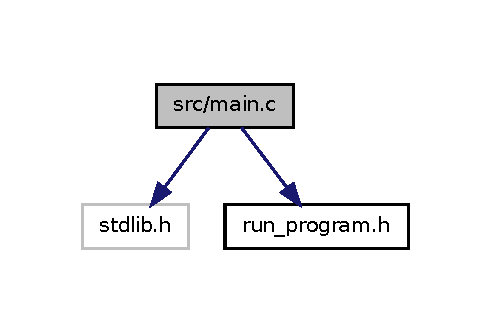
\includegraphics[width=236pt]{main_8c__incl}
\end{center}
\end{figure}
\subsection*{Functions}
\begin{DoxyCompactItemize}
\item 
int \hyperlink{main_8c_a3c04138a5bfe5d72780bb7e82a18e627}{main} (int argc, char $\ast$$\ast$argv)
\begin{DoxyCompactList}\small\item\em The \hyperlink{main_8c_a3c04138a5bfe5d72780bb7e82a18e627}{main()} function is only a wrapper for the \hyperlink{run__program_8c_ac1f545534cdaab9094198a5dc2c2a79f}{run()} function. \item\end{DoxyCompactList}\end{DoxyCompactItemize}


\subsection{Function Documentation}
\hypertarget{main_8c_a3c04138a5bfe5d72780bb7e82a18e627}{
\index{main.c@{main.c}!main@{main}}
\index{main@{main}!main.c@{main.c}}
\subsubsection[{main}]{\setlength{\rightskip}{0pt plus 5cm}int main (
\begin{DoxyParamCaption}
\item[{int}]{ argc, }
\item[{char $\ast$$\ast$}]{ argv}
\end{DoxyParamCaption}
)}}
\label{main_8c_a3c04138a5bfe5d72780bb7e82a18e627}


The \hyperlink{main_8c_a3c04138a5bfe5d72780bb7e82a18e627}{main()} function is only a wrapper for the \hyperlink{run__program_8c_ac1f545534cdaab9094198a5dc2c2a79f}{run()} function. 

The \hyperlink{main_8c_a3c04138a5bfe5d72780bb7e82a18e627}{main()} function only calls \hyperlink{run__program_8c_ac1f545534cdaab9094198a5dc2c2a79f}{run()}. This is because \hyperlink{main_8c_a3c04138a5bfe5d72780bb7e82a18e627}{main()} itself cannot be unit-\/tested with check. Therefore the real work is done by \hyperlink{run__program_8c_ac1f545534cdaab9094198a5dc2c2a79f}{run()}.


\begin{DoxyParams}{Parameters}
\item[\mbox{\tt[in]} {\em argc}]Number of command line arguments \item[\mbox{\tt[in]} {\em argv}]Array of all command line arguments \end{DoxyParams}
\begin{DoxyReturn}{Returns}
EXIT\_\-SUCCESS $|$ EXIT\_\-FAILURE 
\end{DoxyReturn}
\begin{DoxySeeAlso}{See also}
info check 
\end{DoxySeeAlso}


Definition at line 27 of file main.c.




\begin{DoxyCode}
{
    int exit_value = EXIT_FAILURE;

    exit_value = run( argc, argv );

    return exit_value;
}
\end{DoxyCode}



\hypertarget{run__program_8c}{
\section{src/run\_\-program.c File Reference}
\label{run__program_8c}\index{src/run\_\-program.c@{src/run\_\-program.c}}
}
{\ttfamily \#include $<$unistd.h$>$}\par
{\ttfamily \#include $<$stdio.h$>$}\par
{\ttfamily \#include $<$stdlib.h$>$}\par
{\ttfamily \#include $<$string.h$>$}\par
{\ttfamily \#include $<$ctype.h$>$}\par
{\ttfamily \#include $<$stdbool.h$>$}\par
{\ttfamily \#include \char`\"{}global\_\-const.h\char`\"{}}\par
{\ttfamily \#include \char`\"{}run\_\-program.h\char`\"{}}\par
{\ttfamily \#include \char`\"{}io.h\char`\"{}}\par
{\ttfamily \#include \char`\"{}board.h\char`\"{}}\par
{\ttfamily \#include \char`\"{}global\_\-tools.h\char`\"{}}\par
Include dependency graph for run\_\-program.c:\nopagebreak
\begin{figure}[H]
\begin{center}
\leavevmode
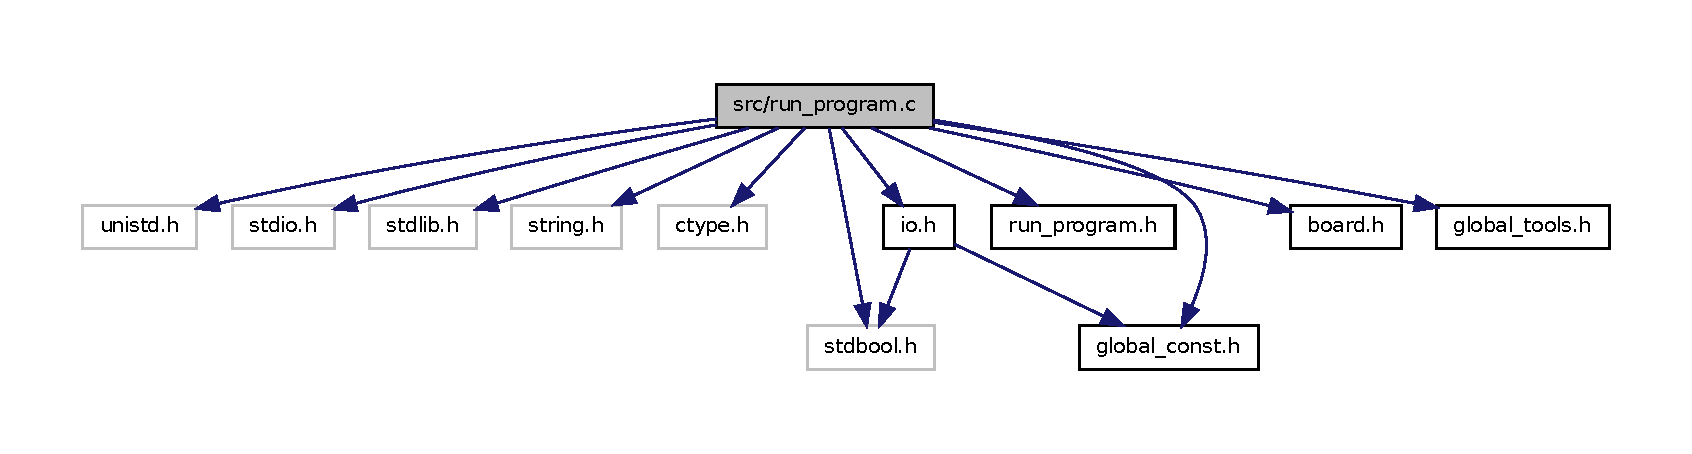
\includegraphics[width=400pt]{run__program_8c__incl}
\end{center}
\end{figure}
\subsection*{Data Structures}
\begin{DoxyCompactItemize}
\item 
struct \hyperlink{structcommand__func}{command\_\-func}
\begin{DoxyCompactList}\small\item\em Connects one given command name with proper function pointer. \item\end{DoxyCompactList}\end{DoxyCompactItemize}
\subsection*{Functions}
\begin{DoxyCompactItemize}
\item 
void \hyperlink{run__program_8c_a4c6d2b52cb37198b390becc56f1e6142}{init\_\-known\_\-commands} (void)
\begin{DoxyCompactList}\small\item\em Initializes all known GTP commands. \item\end{DoxyCompactList}\item 
void \hyperlink{run__program_8c_a040c01612cc61fa6d082f246f07a22e4}{read\_\-opts} (int argc, char $\ast$$\ast$argv)
\begin{DoxyCompactList}\small\item\em Parses command line arguments. \item\end{DoxyCompactList}\item 
void \hyperlink{run__program_8c_a11413e5c3a3a9450976eb102a7c07c20}{select\_\-command} (struct \hyperlink{structcommand}{command} $\ast$command\_\-data)
\begin{DoxyCompactList}\small\item\em Selects the function that is associated with a certain GTP command. \item\end{DoxyCompactList}\item 
void \hyperlink{run__program_8c_a6fd979873dac5f05f7554345f9ca92bb}{print\_\-help\_\-message} (void)
\begin{DoxyCompactList}\small\item\em Prints help message to STDOT. \item\end{DoxyCompactList}\item 
void \hyperlink{run__program_8c_ac6230d495fc909bb61195c45f703d492}{print\_\-version} (void)
\begin{DoxyCompactList}\small\item\em Prints name and version number to STDOUT. \item\end{DoxyCompactList}\item 
void \hyperlink{run__program_8c_a1e1c6b03caa51f0c2aa5879f82be64c9}{set\_\-quit\_\-program} (void)
\begin{DoxyCompactList}\small\item\em Sets control variable for working loop. \item\end{DoxyCompactList}\item 
void \hyperlink{group___g_t_p___administrative___commands_ga57d397237b5bc6129ada6cdcfeaa9aad}{gtp\_\-protocol\_\-version} (int gtp\_\-argc, char gtp\_\-argv\mbox{[}$\,$\mbox{]}\mbox{[}MAX\_\-TOKEN\_\-LENGTH\mbox{]})
\begin{DoxyCompactList}\small\item\em Shows the used GTP version number. \item\end{DoxyCompactList}\item 
void \hyperlink{group___g_t_p___administrative___commands_ga493e544f8b83dd08fb5ebf25c127fb60}{gtp\_\-name} (int gtp\_\-argc, char gtp\_\-argv\mbox{[}$\,$\mbox{]}\mbox{[}MAX\_\-TOKEN\_\-LENGTH\mbox{]})
\begin{DoxyCompactList}\small\item\em Shows the program's name. \item\end{DoxyCompactList}\item 
void \hyperlink{group___g_t_p___administrative___commands_ga264cb45ac6de56306d1006a4ee8a1f4d}{gtp\_\-version} (int gtp\_\-argc, char gtp\_\-argv\mbox{[}$\,$\mbox{]}\mbox{[}MAX\_\-TOKEN\_\-LENGTH\mbox{]})
\begin{DoxyCompactList}\small\item\em Shows the program's version number. \item\end{DoxyCompactList}\item 
void \hyperlink{group___g_t_p___administrative___commands_gac1f9e22691e53c8b8aa46d473008c262}{gtp\_\-known\_\-command} (int gtp\_\-argc, char gtp\_\-argv\mbox{[}$\,$\mbox{]}\mbox{[}MAX\_\-TOKEN\_\-LENGTH\mbox{]})
\begin{DoxyCompactList}\small\item\em Shows whether a given GTP command is implemented or not. \item\end{DoxyCompactList}\item 
void \hyperlink{group___g_t_p___administrative___commands_gabe46d9c2f68c87415a2550ec8358c664}{gtp\_\-list\_\-commands} (int gtp\_\-argc, char gtp\_\-argv\mbox{[}$\,$\mbox{]}\mbox{[}MAX\_\-TOKEN\_\-LENGTH\mbox{]})
\begin{DoxyCompactList}\small\item\em Shows a list of all know GTP commands. \item\end{DoxyCompactList}\item 
void \hyperlink{group___g_t_p___administrative___commands_ga625849e565ca8f4e13fc521165d73910}{gtp\_\-quit} (int gtp\_\-argc, char gtp\_\-argv\mbox{[}$\,$\mbox{]}\mbox{[}MAX\_\-TOKEN\_\-LENGTH\mbox{]})
\begin{DoxyCompactList}\small\item\em Quits the program. \item\end{DoxyCompactList}\item 
void \hyperlink{group___g_t_p___setup___commands_ga79e2fa5bdce2dd440754746a2e35dd24}{gtp\_\-boardsize} (int gtp\_\-argc, char gtp\_\-argv\mbox{[}$\,$\mbox{]}\mbox{[}MAX\_\-TOKEN\_\-LENGTH\mbox{]})
\begin{DoxyCompactList}\small\item\em Changes the current board size. \item\end{DoxyCompactList}\item 
void \hyperlink{group___g_t_p___setup___commands_ga2a539d6423ba407b126487e12a6a222b}{gtp\_\-clear\_\-board} (int gtp\_\-argc, char gtp\_\-argv\mbox{[}$\,$\mbox{]}\mbox{[}MAX\_\-TOKEN\_\-LENGTH\mbox{]})
\begin{DoxyCompactList}\small\item\em Clears the board. \item\end{DoxyCompactList}\item 
void \hyperlink{group___g_t_p___setup___commands_ga9f823dc0dc9c21fabf4ba223fc515682}{gtp\_\-komi} (int gtp\_\-argc, char gtp\_\-argv\mbox{[}$\,$\mbox{]}\mbox{[}MAX\_\-TOKEN\_\-LENGTH\mbox{]})
\begin{DoxyCompactList}\small\item\em Sets komi. \item\end{DoxyCompactList}\item 
void \hyperlink{group___g_t_p___core___play___commands_ga16a060c01868977200be0b381b03c6f9}{gtp\_\-play} (int gtp\_\-argc, char gtp\_\-argv\mbox{[}$\,$\mbox{]}\mbox{[}MAX\_\-TOKEN\_\-LENGTH\mbox{]})
\begin{DoxyCompactList}\small\item\em Description missing! \item\end{DoxyCompactList}\item 
void \hyperlink{group___g_t_p___debug___commands_ga7c297f28150386dc85b1de08e6f8d456}{gtp\_\-showboard} (int gtp\_\-argc, char gtp\_\-argv\mbox{[}$\,$\mbox{]}\mbox{[}MAX\_\-TOKEN\_\-LENGTH\mbox{]})
\begin{DoxyCompactList}\small\item\em Shows a simple ASCII board. \item\end{DoxyCompactList}\item 
int \hyperlink{run__program_8c_ac1f545534cdaab9094198a5dc2c2a79f}{run} (int argc, char $\ast$$\ast$argv)
\begin{DoxyCompactList}\small\item\em Substitute for \hyperlink{main_8c_a3c04138a5bfe5d72780bb7e82a18e627}{main()} function, because \hyperlink{main_8c_a3c04138a5bfe5d72780bb7e82a18e627}{main()} itself cannot be unit-\/tested with check. \item\end{DoxyCompactList}\end{DoxyCompactItemize}
\subsection*{Variables}
\begin{DoxyCompactItemize}
\item 
const char \hyperlink{run__program_8c_a4fad729e0a45065b0ff24a81d7e0173d}{help\_\-message} \mbox{[}$\,$\mbox{]}
\begin{DoxyCompactList}\small\item\em The default help message shown with -\/h. \item\end{DoxyCompactList}\item 
int \hyperlink{run__program_8c_a8573b61fb976af69bdabd11cf835d9c6}{quit\_\-program} = 0
\begin{DoxyCompactList}\small\item\em If set to 1 the main control loop exits. \item\end{DoxyCompactList}\item 
struct \hyperlink{structcommand__func}{command\_\-func} \hyperlink{run__program_8c_a0cc8ce41f59759415b395e6797dc67aa}{known\_\-commands} \mbox{[}COUNT\_\-KNOWN\_\-COMMANDS\mbox{]}
\begin{DoxyCompactList}\small\item\em Array of known (implemented) commands. \item\end{DoxyCompactList}\item 
float \hyperlink{run__program_8c_a65723173a5e578c1acff2b1790e5c579}{komi} = 0.0
\begin{DoxyCompactList}\small\item\em The current komi value. \item\end{DoxyCompactList}\end{DoxyCompactItemize}


\subsection{Function Documentation}
\hypertarget{run__program_8c_a4c6d2b52cb37198b390becc56f1e6142}{
\index{run\_\-program.c@{run\_\-program.c}!init\_\-known\_\-commands@{init\_\-known\_\-commands}}
\index{init\_\-known\_\-commands@{init\_\-known\_\-commands}!run_program.c@{run\_\-program.c}}
\subsubsection[{init\_\-known\_\-commands}]{\setlength{\rightskip}{0pt plus 5cm}void init\_\-known\_\-commands (
\begin{DoxyParamCaption}
\item[{void}]{}
\end{DoxyParamCaption}
)}}
\label{run__program_8c_a4c6d2b52cb37198b390becc56f1e6142}


Initializes all known GTP commands. 

Initializes a data structure for all implemented GTP commands. The data structure is an array of pairs of names and function pointers.

\begin{DoxyReturn}{Returns}
nothing 
\end{DoxyReturn}
\begin{DoxySeeAlso}{See also}
\mbox{[}n/a\mbox{]} 
\end{DoxySeeAlso}


Definition at line 216 of file run\_\-program.c.




\begin{DoxyCode}
{
    int i = 0;

    my_strcpy( known_commands[i].command, "protocol_version", MAX_TOKEN_LENGTH );
      
    known_commands[i++].function = (*gtp_protocol_version);
    my_strcpy( known_commands[i].command, "name", MAX_TOKEN_LENGTH );
    known_commands[i++].function = (*gtp_name);
    my_strcpy( known_commands[i].command, "version", MAX_TOKEN_LENGTH );
    known_commands[i++].function = (*gtp_version);
    my_strcpy( known_commands[i].command, "known_command", MAX_TOKEN_LENGTH );
    known_commands[i++].function = (*gtp_known_command);
    my_strcpy( known_commands[i].command, "list_commands", MAX_TOKEN_LENGTH );
    known_commands[i++].function = (*gtp_list_commands);
    my_strcpy( known_commands[i].command, "quit", MAX_TOKEN_LENGTH );
    known_commands[i++].function = (*gtp_quit);
    my_strcpy( known_commands[i].command, "boardsize", MAX_TOKEN_LENGTH );
    known_commands[i++].function = (*gtp_boardsize);
    my_strcpy( known_commands[i].command, "clear_board", MAX_TOKEN_LENGTH );
    known_commands[i++].function = (*gtp_clear_board);
    my_strcpy( known_commands[i].command, "komi", MAX_TOKEN_LENGTH );
    known_commands[i++].function = (*gtp_komi);
    my_strcpy( known_commands[i].command, "play", MAX_TOKEN_LENGTH );
    known_commands[i++].function = (*gtp_play);
    my_strcpy( known_commands[i].command, "showboard", MAX_TOKEN_LENGTH );
    known_commands[i++].function = (*gtp_showboard);

    if ( i != COUNT_KNOWN_COMMANDS ) {
        fprintf(
            stdout
          , "Commands implemented: %d\nCOUNT_KNOWN_COMMANDS: %d\n"
          , i, COUNT_KNOWN_COMMANDS
        );
        exit(1);
    }

    return;
}
\end{DoxyCode}


\hypertarget{run__program_8c_a6fd979873dac5f05f7554345f9ca92bb}{
\index{run\_\-program.c@{run\_\-program.c}!print\_\-help\_\-message@{print\_\-help\_\-message}}
\index{print\_\-help\_\-message@{print\_\-help\_\-message}!run_program.c@{run\_\-program.c}}
\subsubsection[{print\_\-help\_\-message}]{\setlength{\rightskip}{0pt plus 5cm}void print\_\-help\_\-message (
\begin{DoxyParamCaption}
\item[{void}]{}
\end{DoxyParamCaption}
)}}
\label{run__program_8c_a6fd979873dac5f05f7554345f9ca92bb}


Prints help message to STDOT. 

\hyperlink{run__program_8c_a6fd979873dac5f05f7554345f9ca92bb}{print\_\-help\_\-message()} prints a help message to STDOUT. The help message itself is defined in help\_\-message. This function is called when the command line paramter -\/h is set.

\begin{DoxyReturn}{Returns}
nothing 
\end{DoxyReturn}
\begin{DoxySeeAlso}{See also}
\mbox{[}n/a\mbox{]} 
\end{DoxySeeAlso}


Definition at line 179 of file run\_\-program.c.




\begin{DoxyCode}
{

    printf( "%s", help_message );

    return;
}
\end{DoxyCode}


\hypertarget{run__program_8c_ac6230d495fc909bb61195c45f703d492}{
\index{run\_\-program.c@{run\_\-program.c}!print\_\-version@{print\_\-version}}
\index{print\_\-version@{print\_\-version}!run_program.c@{run\_\-program.c}}
\subsubsection[{print\_\-version}]{\setlength{\rightskip}{0pt plus 5cm}void print\_\-version (
\begin{DoxyParamCaption}
\item[{void}]{}
\end{DoxyParamCaption}
)}}
\label{run__program_8c_ac6230d495fc909bb61195c45f703d492}


Prints name and version number to STDOUT. 

\hyperlink{run__program_8c_ac6230d495fc909bb61195c45f703d492}{print\_\-version()} prints the name aof the program and its version number of the program to STDOUT. The name is defined in PROGRAM\_\-NAME, the version is defined in PROGRAM\_\-VERSION. This function is called when the command line parameter -\/v is set.

\begin{DoxyReturn}{Returns}
nothing 
\end{DoxyReturn}
\begin{DoxySeeAlso}{See also}
\mbox{[}n/a\mbox{]} 
\end{DoxySeeAlso}


Definition at line 199 of file run\_\-program.c.




\begin{DoxyCode}
{

    printf( "%s %s\n", PROGRAM_NAME, PROGRAM_VERSION );

    return;
}
\end{DoxyCode}


\hypertarget{run__program_8c_a040c01612cc61fa6d082f246f07a22e4}{
\index{run\_\-program.c@{run\_\-program.c}!read\_\-opts@{read\_\-opts}}
\index{read\_\-opts@{read\_\-opts}!run_program.c@{run\_\-program.c}}
\subsubsection[{read\_\-opts}]{\setlength{\rightskip}{0pt plus 5cm}void read\_\-opts (
\begin{DoxyParamCaption}
\item[{int}]{ argc, }
\item[{char $\ast$$\ast$}]{ argv}
\end{DoxyParamCaption}
)}}
\label{run__program_8c_a040c01612cc61fa6d082f246f07a22e4}


Parses command line arguments. 

\hyperlink{run__program_8c_a040c01612cc61fa6d082f246f07a22e4}{read\_\-opts()} parses the command line arguments with which the program has been started. ( Do not confuse these with the arguments given to a GTP command. ) For certain arguments -\/-\/ like -\/h or -\/v -\/-\/ the appropriate function is called.


\begin{DoxyParams}{Parameters}
\item[\mbox{\tt[in]} {\em argc}]Number of arguments (same as for \hyperlink{main_8c_a3c04138a5bfe5d72780bb7e82a18e627}{main()}) \item[\mbox{\tt[in]} {\em argv}]Array of arguments (same as for \hyperlink{main_8c_a3c04138a5bfe5d72780bb7e82a18e627}{main()}) \end{DoxyParams}
\begin{DoxyReturn}{Returns}
nothing 
\end{DoxyReturn}
\begin{DoxySeeAlso}{See also}
man 3 getopt 
\end{DoxySeeAlso}


Definition at line 147 of file run\_\-program.c.




\begin{DoxyCode}
{
    int opt;

    while ( ( opt = getopt( argc, argv, VALID_OPTIONS ) ) != -1 ) {
        switch (opt) {
            case 'h':
                print_help_message();
                set_quit_program();
                break;
            case 'v':
                print_version();
                set_quit_program();
                break;
            default:
                exit(EXIT_FAILURE);
        }
    }

    return;
}
\end{DoxyCode}


\hypertarget{run__program_8c_ac1f545534cdaab9094198a5dc2c2a79f}{
\index{run\_\-program.c@{run\_\-program.c}!run@{run}}
\index{run@{run}!run_program.c@{run\_\-program.c}}
\subsubsection[{run}]{\setlength{\rightskip}{0pt plus 5cm}int run (
\begin{DoxyParamCaption}
\item[{int}]{ argc, }
\item[{char $\ast$$\ast$}]{ argv}
\end{DoxyParamCaption}
)}}
\label{run__program_8c_ac1f545534cdaab9094198a5dc2c2a79f}


Substitute for \hyperlink{main_8c_a3c04138a5bfe5d72780bb7e82a18e627}{main()} function, because \hyperlink{main_8c_a3c04138a5bfe5d72780bb7e82a18e627}{main()} itself cannot be unit-\/tested with check. 

The \hyperlink{run__program_8c_ac1f545534cdaab9094198a5dc2c2a79f}{run()} function performs the following tasks:
\begin{DoxyEnumerate}
\item Initialization
\item STDOUT buffer size set to NULL
\item Checking command line arguments (like -\/h, -\/v, etc.)
\item Starting the working loop
\end{DoxyEnumerate}


\begin{DoxyParams}{Parameters}
\item[\mbox{\tt[in]} {\em argc}]Number of command line arguments (same as for \hyperlink{main_8c_a3c04138a5bfe5d72780bb7e82a18e627}{main()}). \item[\mbox{\tt[in]} {\em argv}]Array of all command line arguments (same as for \hyperlink{main_8c_a3c04138a5bfe5d72780bb7e82a18e627}{main()}). \end{DoxyParams}
\begin{DoxyReturn}{Returns}
EXIT\_\-SUCCESS $|$ EXIT\_\-FAILURE 
\end{DoxyReturn}
\begin{DoxySeeAlso}{See also}
info check 
\end{DoxySeeAlso}


Definition at line 80 of file run\_\-program.c.




\begin{DoxyCode}
{
    struct command command_data;

    // Initialization
    init_board(BOARD_SIZE_DEFAULT);
    init_known_commands();

    // STDOUT must be unbuffered:
    setbuf( stdout, NULL );

    // Read command line arguments:
    read_opts( argc, argv );

    // Working loop:
    while ( quit_program == 0 ) {
        read_gtp_input(&command_data);

        // Ignore empty lines:
        if ( is_input_empty() == true ) {
            continue;
        }

        if ( get_output_error() == false ) {
            select_command(&command_data);
        }

        print_output(command_data.id);
    }

    free_board();

    return EXIT_SUCCESS;
}
\end{DoxyCode}


\hypertarget{run__program_8c_a11413e5c3a3a9450976eb102a7c07c20}{
\index{run\_\-program.c@{run\_\-program.c}!select\_\-command@{select\_\-command}}
\index{select\_\-command@{select\_\-command}!run_program.c@{run\_\-program.c}}
\subsubsection[{select\_\-command}]{\setlength{\rightskip}{0pt plus 5cm}void select\_\-command (
\begin{DoxyParamCaption}
\item[{struct {\bf command} $\ast$}]{ command\_\-data}
\end{DoxyParamCaption}
)}}
\label{run__program_8c_a11413e5c3a3a9450976eb102a7c07c20}


Selects the function that is associated with a certain GTP command. 

\hyperlink{run__program_8c_a11413e5c3a3a9450976eb102a7c07c20}{select\_\-command()} receives a comman data structure and calls the function which is associated with this GTP command.


\begin{DoxyParams}{Parameters}
\item[\mbox{\tt[in]} {\em $\ast$command\_\-data}]struct command \end{DoxyParams}
\begin{DoxyReturn}{Returns}
nothing 
\end{DoxyReturn}
\begin{DoxySeeAlso}{See also}
\mbox{[}n/a\mbox{]} 
\end{DoxySeeAlso}


Definition at line 265 of file run\_\-program.c.




\begin{DoxyCode}
{
    int  i;
    bool is_command = false;

    for ( i = 0; i < COUNT_KNOWN_COMMANDS; i++ ) {
        if ( strcmp( known_commands[i].command, command_data->name ) == 0 ) {
            is_command = true;
            known_commands[i].function( command_data->gtp_argc, command_data->
      gtp_argv );
            break;
        }
    }

    if ( is_command == false ) {
        set_output_error();
        add_output("unknown command");
    }

    return;
}
\end{DoxyCode}


\hypertarget{run__program_8c_a1e1c6b03caa51f0c2aa5879f82be64c9}{
\index{run\_\-program.c@{run\_\-program.c}!set\_\-quit\_\-program@{set\_\-quit\_\-program}}
\index{set\_\-quit\_\-program@{set\_\-quit\_\-program}!run_program.c@{run\_\-program.c}}
\subsubsection[{set\_\-quit\_\-program}]{\setlength{\rightskip}{0pt plus 5cm}void set\_\-quit\_\-program (
\begin{DoxyParamCaption}
\item[{void}]{}
\end{DoxyParamCaption}
)}}
\label{run__program_8c_a1e1c6b03caa51f0c2aa5879f82be64c9}


Sets control variable for working loop. 

The \hyperlink{run__program_8c_a1e1c6b03caa51f0c2aa5879f82be64c9}{set\_\-quit\_\-program()} function sets the variable quit\_\-program to 1. When this variable is 1, the control loop stops and the program exits.

\begin{DoxyReturn}{Returns}
nothing 
\end{DoxyReturn}
\begin{DoxySeeAlso}{See also}
\mbox{[}n/a\mbox{]} 
\end{DoxySeeAlso}


Definition at line 126 of file run\_\-program.c.




\begin{DoxyCode}
{

    quit_program = 1;

    return;
}
\end{DoxyCode}




\subsection{Variable Documentation}
\hypertarget{run__program_8c_a4fad729e0a45065b0ff24a81d7e0173d}{
\index{run\_\-program.c@{run\_\-program.c}!help\_\-message@{help\_\-message}}
\index{help\_\-message@{help\_\-message}!run_program.c@{run\_\-program.c}}
\subsubsection[{help\_\-message}]{\setlength{\rightskip}{0pt plus 5cm}const char {\bf help\_\-message}\mbox{[}$\,$\mbox{]}}}
\label{run__program_8c_a4fad729e0a45065b0ff24a81d7e0173d}
{\bfseries Initial value:}
\begin{DoxyCode}
"This is a placeholder for the help message.\n\
This message is shown when the program is called\n\
with the command line argument -h.\n"
\end{DoxyCode}


The default help message shown with -\/h. 



Definition at line 15 of file run\_\-program.c.

\hypertarget{run__program_8c_a0cc8ce41f59759415b395e6797dc67aa}{
\index{run\_\-program.c@{run\_\-program.c}!known\_\-commands@{known\_\-commands}}
\index{known\_\-commands@{known\_\-commands}!run_program.c@{run\_\-program.c}}
\subsubsection[{known\_\-commands}]{\setlength{\rightskip}{0pt plus 5cm}struct {\bf command\_\-func} {\bf known\_\-commands}\mbox{[}COUNT\_\-KNOWN\_\-COMMANDS\mbox{]}}}
\label{run__program_8c_a0cc8ce41f59759415b395e6797dc67aa}


Array of known (implemented) commands. 



Definition at line 31 of file run\_\-program.c.

\hypertarget{run__program_8c_a65723173a5e578c1acff2b1790e5c579}{
\index{run\_\-program.c@{run\_\-program.c}!komi@{komi}}
\index{komi@{komi}!run_program.c@{run\_\-program.c}}
\subsubsection[{komi}]{\setlength{\rightskip}{0pt plus 5cm}float {\bf komi} = 0.0}}
\label{run__program_8c_a65723173a5e578c1acff2b1790e5c579}


The current komi value. 



Definition at line 34 of file run\_\-program.c.

\hypertarget{run__program_8c_a8573b61fb976af69bdabd11cf835d9c6}{
\index{run\_\-program.c@{run\_\-program.c}!quit\_\-program@{quit\_\-program}}
\index{quit\_\-program@{quit\_\-program}!run_program.c@{run\_\-program.c}}
\subsubsection[{quit\_\-program}]{\setlength{\rightskip}{0pt plus 5cm}int {\bf quit\_\-program} = 0}}
\label{run__program_8c_a8573b61fb976af69bdabd11cf835d9c6}


If set to 1 the main control loop exits. 



Definition at line 21 of file run\_\-program.c.


\hypertarget{run__program_8h}{
\section{src/run\_\-program.h File Reference}
\label{run__program_8h}\index{src/run\_\-program.h@{src/run\_\-program.h}}
}
This graph shows which files directly or indirectly include this file:\nopagebreak
\begin{figure}[H]
\begin{center}
\leavevmode
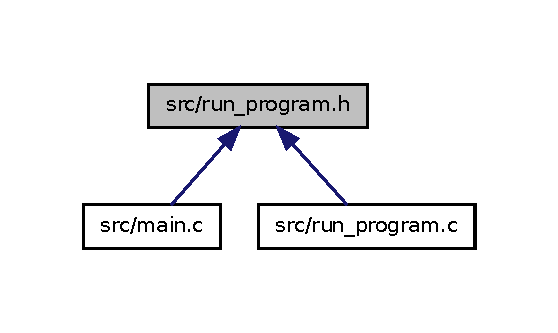
\includegraphics[width=268pt]{run__program_8h__dep__incl}
\end{center}
\end{figure}
\subsection*{Defines}
\begin{DoxyCompactItemize}
\item 
\#define \hyperlink{run__program_8h_a713840100e793ae1f2587d5abbf635ee}{COUNT\_\-KNOWN\_\-COMMANDS}~11
\begin{DoxyCompactList}\small\item\em Defines the number of known GTP commands. \item\end{DoxyCompactList}\end{DoxyCompactItemize}
\subsection*{Functions}
\begin{DoxyCompactItemize}
\item 
int \hyperlink{run__program_8h_ac1f545534cdaab9094198a5dc2c2a79f}{run} (int argc, char $\ast$$\ast$argv)
\begin{DoxyCompactList}\small\item\em Substitute for \hyperlink{main_8c_a3c04138a5bfe5d72780bb7e82a18e627}{main()} function, because \hyperlink{main_8c_a3c04138a5bfe5d72780bb7e82a18e627}{main()} itself cannot be unit-\/tested with check. \item\end{DoxyCompactList}\end{DoxyCompactItemize}


\subsection{Define Documentation}
\hypertarget{run__program_8h_a713840100e793ae1f2587d5abbf635ee}{
\index{run\_\-program.h@{run\_\-program.h}!COUNT\_\-KNOWN\_\-COMMANDS@{COUNT\_\-KNOWN\_\-COMMANDS}}
\index{COUNT\_\-KNOWN\_\-COMMANDS@{COUNT\_\-KNOWN\_\-COMMANDS}!run_program.h@{run\_\-program.h}}
\subsubsection[{COUNT\_\-KNOWN\_\-COMMANDS}]{\setlength{\rightskip}{0pt plus 5cm}\#define COUNT\_\-KNOWN\_\-COMMANDS~11}}
\label{run__program_8h_a713840100e793ae1f2587d5abbf635ee}


Defines the number of known GTP commands. 



Definition at line 5 of file run\_\-program.h.



\subsection{Function Documentation}
\hypertarget{run__program_8h_ac1f545534cdaab9094198a5dc2c2a79f}{
\index{run\_\-program.h@{run\_\-program.h}!run@{run}}
\index{run@{run}!run_program.h@{run\_\-program.h}}
\subsubsection[{run}]{\setlength{\rightskip}{0pt plus 5cm}int run (
\begin{DoxyParamCaption}
\item[{int}]{ argc, }
\item[{char $\ast$$\ast$}]{ argv}
\end{DoxyParamCaption}
)}}
\label{run__program_8h_ac1f545534cdaab9094198a5dc2c2a79f}


Substitute for \hyperlink{main_8c_a3c04138a5bfe5d72780bb7e82a18e627}{main()} function, because \hyperlink{main_8c_a3c04138a5bfe5d72780bb7e82a18e627}{main()} itself cannot be unit-\/tested with check. 

The \hyperlink{run__program_8c_ac1f545534cdaab9094198a5dc2c2a79f}{run()} function performs the following tasks:
\begin{DoxyEnumerate}
\item Initialization
\item STDOUT buffer size set to NULL
\item Checking command line arguments (like -\/h, -\/v, etc.)
\item Starting the working loop
\end{DoxyEnumerate}


\begin{DoxyParams}{Parameters}
\item[\mbox{\tt[in]} {\em argc}]Number of command line arguments (same as for \hyperlink{main_8c_a3c04138a5bfe5d72780bb7e82a18e627}{main()}). \item[\mbox{\tt[in]} {\em argv}]Array of all command line arguments (same as for \hyperlink{main_8c_a3c04138a5bfe5d72780bb7e82a18e627}{main()}). \end{DoxyParams}
\begin{DoxyReturn}{Returns}
EXIT\_\-SUCCESS $|$ EXIT\_\-FAILURE 
\end{DoxyReturn}
\begin{DoxySeeAlso}{See also}
info check 
\end{DoxySeeAlso}


Definition at line 80 of file run\_\-program.c.




\begin{DoxyCode}
{
    struct command command_data;

    // Initialization
    init_board(BOARD_SIZE_DEFAULT);
    init_known_commands();

    // STDOUT must be unbuffered:
    setbuf( stdout, NULL );

    // Read command line arguments:
    read_opts( argc, argv );

    // Working loop:
    while ( quit_program == 0 ) {
        read_gtp_input(&command_data);

        // Ignore empty lines:
        if ( is_input_empty() == true ) {
            continue;
        }

        if ( get_output_error() == false ) {
            select_command(&command_data);
        }

        print_output(command_data.id);
    }

    free_board();

    return EXIT_SUCCESS;
}
\end{DoxyCode}



\printindex
\end{document}
